\documentclass[11pt, letterpaper]{memoir}
\usepackage[plainpages=false, colorlinks, urlcolor=black, citecolor=black,
	linkcolor=blue]{hyperref}
\usepackage{graphicx}
\usepackage[utf8]{inputenc}
\usepackage{txfonts}
\usepackage{listings}
\usepackage{multirow}
\usepackage[spanish, english]{babel}
%\usepackage[dvips]{epsfig}
%\usepackage{epsfig}
%\usepackage{psfig}

%% Margenes segun Normas
%% Ancho Legal 21,59cm /  8,5in
%% Alto  Legal 33,02cm / 13,0in
\paperheight    27.81cm % alto letter
\paperwidth     21.59cm % ancho
\hoffset        -1.0in % Seteo a 0 el margen izquierdo
\voffset        -1.0in % Seteo a 0 el margen superior
\oddsidemargin  3.80cm % Margen izquierdo (pag. impar)
% \evensidemargin 2.55cm % Margen izquierdo (pag. par) Acrobat Winkk
\evensidemargin 2.59cm % Margen izquierdo (pag. par)
\topmargin      1.00cm % Margen superior
\headheight     5.00mm % Ancho encabezado
\headsep        8.00mm % Separacion encabezado-cuerpo
\textheight     23.5cm % Alto cuerpo
\textwidth      15.2cm % Ancho cuerpo
\footskip       1.30cm % Separacion piepag-cuerpo
\parindent      0em
\parskip        1ex

\lstloadlanguages{C++, sh, IDL, make}
\lstset{basicstyle=\small\sffamily, commentstyle=\slshape,
        numbers=left, numberstyle=\tiny, numbersep=10pt,
        extendedchars, frame=lines,
        floatplacement=ht, captionpos=b,
        defaultdialect=[CORBA]IDL}

\title{Data Distribution Service as an alternative to
the CORBA Notification Service for Alma Common Software}
\author{Jorge Avarias}

\newcommand{\doctitle}{A NEW SCHEDULING ALGORITHM FOR ALMA OBSERVATORY}

\begin{document}
\selectlanguage{english}
\begin{titlingpage}
\begin{center}
  \begin{tabular}{c}
    \hspace{0.2cm}
    \begin{tabular}{c}
        \LARGE{UNIVERSIDAD T\'ECNICA FEDERICO SANTA MAR\'IA}\\
        \LARGE{DEPARTAMENTO DE INFORM\'ATICA}\\
        \LARGE{SANTIAGO -- CHILE}\\
        \hspace{8.0cm}
        %\vspace{1.2cm}
    \end{tabular}
    \hspace{0.2cm}
  \end{tabular}

  \begin{figure*}[h!]
  \begin{center}
  
\includegraphics[height=3cm]{images/utfsm}
  \end{center}
  %
\epsfig{file=images/utfsm.eps,height=3cm}
  \end{figure*}

  \vspace{2.0cm}

  \LARGE{\doctitle}

  \vspace{1.0cm}

  \LARGE{JORGE ALEJANDRO AVARIAS ALFARO}

  \Large{\href{mailto:javarias@inf.utfsm.cl}{javarias@inf.utfsm.cl}}

  \vspace{1.0cm}

  \LARGE{TESIS PRESENTADA COMO REQUERIMIENTO PARCIAL PARA OPTAR AL GRADO DE\\
         MAG\'ISTER EN CIENCIAS DE LA INGENIR\'IA INFORM\'ATICA}

  \vspace{1.5cm}

  \normalsize{}

%  \textbf{PROFESOR GU\'IA:  }

  %\vspace{0.3cm}

  \vspace{0.5cm}

%  \textbf{PROFESOR CORREFERENTE:  JAVIER CA\~NAS}

  %\vspace{0.3cm}
\end{center}

\vfill \centering Diciembre -- 2008

\end{titlingpage}

\thispagestyle{empty}
\bibliographystyle{alpha}
%\maketitle
\frontmatter
%\thispagestyle{empty}
\vspace*{\fill}

\selectlanguage{english}
\begin{center}
\begin{LARGE}\textbf{Abstract}\end{LARGE}
\end{center}

The Atacama Large Millimeter Array (ALMA) is the biggest astronomical project, currently under
construction in the Chilean Atacama desert. This radio-telescope consists of more than 60
antennas, the telescope will be able to observe simultaneously different sky sources, organized in one or more
variable size arrays. The observatory's scheduling system considers full automatic
operation, and dynamic rescheduling of the observations according to factors changing continuously, like atmospheric
conditions, source visibility, technical failures or targets of opportunity.
Currently, ALMA, has a dynamic scheduling algorithm which considers a wide-range of scientific,
instrument and weather constraints and requirements, but multiples issues has been
identified. Newer models provide a fresh perspective of this problem, but they lack of the
scientific background, and they have not been tested in a real world problem.
In this thesis will be proven that, is possible to design and implement a new algorithm for ALMA observatory 
considering the long-term scheduling problem, for what the algorithm will provide a schedule 
for different array configurations within an observing
season. The algorithm will be verified and validated using real data, trying to define a metric based on quality
of the scientific output and instrument usage.

\vspace{0.5cm}

\selectlanguage{spanish}
\begin{center}
\begin{LARGE}\textbf{Resumen}\end{LARGE}
\end{center}

El Atacama Large Millimeter Array (ALMA) es el mayor proyecto astron\'omico actualmente en
construcci\'on en el desierto chileno de Atacama. Este radio-telescopio consiste en m\'as de 60
antenas, que ser\'a capaz de observar simult\'aneamente varias fuentes en el cielo, organizada en una o m\'as arreglos
de tama\~no variable. El sistema de planificaci\'on de observaciones del telescopio
considera una operaci\'on totalmente autom\'atica, y una reprogramaci\'on din\'amica de las tareas de
acuerdo a los factores cambiantes, como las condiciones atmosf\'ericas, visibilidad de la fuente,
fallas t\'ecnicas u objetivos de oportunidad.
Actualmente ALMA tiene un algoritmo de planificaci\'on din\'amica que considera una amplia
gama de restricciones y requerimientos del instrumento cient\'ifico y del clima, sin embargo
m\'ultiples problemas han sido identificados. Los modelos m\'as nuevos ofrecen una nueva
perspectiva de este problema, pero carecen de un trasfondo cient\'ifico y no han sido probados en
un problema del mundo real. Esta tesis probar\'a que es posible dise\~nar e implmentar un nuevo algoritmo para ALMA
teniendo en cuenta el problema de planificaci\'on a largo plazo, donde el algoritmo presentar\'a
un cronograma para las diferentes configuraciones de arreglo disponibles durante una misma
temporada de observaci\'on. El algoritmo se verificar\'a con datos reales, tratando de definir una
m\'etrica basada en la calidad de la producci\'on cient\'ifica y el uso de instrumentos.
\vfill

\cleardoublepage
\selectlanguage{english}
\newpage
\tableofcontents
\cleardoublepage
\listoffigures
\cleardoublepage
\listoftables
\cleardoublepage
\lstlistoflistings

\mainmatter
\cleardoublepage

%\chapter{Introduction}

State-of-the art astronomical facilities are costly to build and operate, it is essential that these facilities be
operated as efficiently as possible maximizing their scientific output. In modern astronomy has been
demonstrated the importance to use automatic modes in the operation of the latest and biggest
telescopes. Over latest decades the problem has attracted more research since new facilities have been
proved that is unfeasible to try to schedule all the observations manually due the complexity to satisfy
the astronomical and the instrumental constraints imposed by the problem and the amount of scientific
proposals to be reviewed. Also due the dynamic nature of some of the constraints like the weather and
the uncertain when an observation is fully complete make this problem more difficult even.

The Atacama Large Millimeter/submillimeter Array (ALMA) is a major collaboration effort between
European, North American and East Asian countries, under construction on the Chilean Chajnantor
plateau, at 5.000 meters altitude. Currently it is the largest radio-telescope on Earth, when completed it
will have 66 antennas of 12 and 7 meters diameter, distributed over a wide extension, with up to 16 kilo-
meters of baseline separation. The ALMA interferometer will provide the possibility to be used as a single
array, or as up to six minor independent arrays or groups of antennas. Over the observing season
multiples arrays configurations will be available changing the antennas position from one place to
another. These places are already defined positions called pads, during normal operations at least two
arrays will be available each of one attached to different correlators computers. As ALMA does not
observe in the visible spectrum, observations are not limited to night time only, thus a 24/7 operation
with as small downtime as possible is expected. However during commissioning operations, ALMA will operate on tied schedules having less than the half of the day-time to do science.

Two different problems have been identified: \textit{``Astronomical observation scheduling problem''} consists on determine a
schedule for the given set of scheduling blocks considering one or more arrays already created in a given
period of time. The idea is to try to observe most of the projects with highest priority in the less amount
of time possible considering all the scientific requirements and constraints; and \textit{``The  Array configuration planning problem''}, what  
is on top of the scheduling array problem. It consists in try to determine a schedule of
observations for the observing season (which is a fixed amount of time and it lasts for several months, up
to 1 year), for given set of the scheduling blocks and the given set the of array configurations. The idea is
to try to observe most of the projects with highest scientific value considering all the scientific
requirements during the observing season, however not all the projects could be completed.

\section{Hypothesis}

ALMA software currently has an algorithm, the Dynamic Scheduling Algorithm implemented as
part of the scheduling subsystem, which does not try optimize the set of selected scheduling unit
as a function of time for long periods of time. Also the algorithm does not try to come up with an
optimal program for array configurations which are given for a season. This algorithm suffers of
serious problems of fairness were it is possible under certain circumstances to get as result a
scheduling unit repeated all over an observation time frame (like a week) letting to starve
projects with the same or higher priority, but belonging to a different participant.
In other hand the most recent model proposal lacks of all astronomical analysis of constraints and
results to decide if the algorithm could be feasible to adapt to the ALMA scheduling requirements
and use into ALMA software.
None of the described methodologies deal with the problem of trying to schedule the proposed
array configurations necessary for the ALMA’s long-term scheduling.

Therefore the hypothesis presented is the following: \textbf{``It is feasible to design and implement an algorithm for the ALMA scheduling problem that can meet most of the astronomical, instrument and weather constraints''}.

\section{Objectives}

\begin{itemize}
\item Develop a new scheduling algorithm that meets the ALMA’s scientific, instrument and
weather constraints, and requirements and successfully integrate it within ALMA software.
The development will be focused in try to solve the long-term scheduling problem, where
the algorithm shall provide a schedule for different array configurations within an
observing season.
\begin{itemize}
\item Study real world constraints gathered from ALMA scheduling requirements.
\item Implement the algorithm in a suitable programming language.
\item Design a model to be applied to the short-term, medium-term and long-term ALMA’s
scheduling problem. Focusing in the long-term problem.
\item Define and develop an algorithm that satisfy the ALMA’s scheduling problem requirements
studied prior.
\item Algorithm must minimize array configuration time, at the same time the number of source
must be maximize. This should minimize the array idle-time.
\end{itemize}
\item Define metrics to evaluate the algorithm performance in terms of idle-time or instrument
usage, scientific performance and completed projects.
\begin{itemize}
\item Metrics must consider idle observatory time and executive time fairness.
\item Develop a suitable test-bench software to evaluate the algorithm.
\item Validate the algorithm using the test-bench.
\end{itemize}
\end{itemize}

\section{Expected results and validation}
The main contribution expected by this work is the implemented algorithm which will be used as
part of the ALMA software for the next years. This would be a significant contribution to the
ALMA project and in general to the astronomical community.
The specific expected results are:
\begin{itemize}
\item An implemented algorithm ready to use in ALMA
\item A suitable test bench to benchmark the performance of the algorithm
\item The output values of the tests done during the validation process. Also the comparison with
another algorithms whenever is possible
\end{itemize}

Since this work mainly considers the performance of an algorithm implementation, the algorithm will be validated
executing performance measurements tests and then comparing these results against previous
studies. This work proposes a new methodology to validate the performance of an observatory
scheduling algorithm hence a full comparison with previous studies could not apply.

The performance tests will be carried over a simulation platform which has been already
developed for ALMA software. The observation projects considered for the test will be real
projects taken from the ALMA’s cycle 2 observing season, however these projects are not publicly
available after a period of time (2 years).

Even when the projects are not publicly available, this shall not affect the thesis results due the
results does not show in detail what project have more chance to be completely observed, the
restriction imposed by ALMA is related to the ability to identify a particularly project and this is
not the purpose of the results that this work will show.

\chapter{State of the art}

\section{Job-shop problem}
The scheduling problem is an optimization problem in which ideal jobs, also called tasks, are assigned to resources at particular times to execute these jobs, the execution of the jobs must satisfy all the constraints, this should be done in a way that the resulting schedule, the solution, is the best possible.

The most well known problem is the \textit{job-shop} scheduling problem presented by first time in 1966 by Graham \cite{graham66}. The objective of this problem is to complete a set jobs, each of which consists of a sequence of actions, where each action has a given duration and might require some resources. The problem is to determine a schedule that minimized the total time required to complete all the jobs, while respecting the resource constraints~\cite{russell03}.

The job-shop dynamic scheduling problem has been researched in the recent years, there are different classifications given to the problem based on the dynamism related to constraints or related to the jobs. A full survey can be found in~\cite{ouelhadj}. Also different methods are discussed to solve the problem.

\section{Fair scheduling: Processor sharing approach}

Another approach to scheduling problem is the proportional fair scheduling studied at level of processor sharing, this problem is very common in computer science and developing of Operating System's kernels~\cite{li09} including real-time systems and in the past, in the 90's was studied in network sharing~\cite{parekh93}. 

In this problem fairness is an essential requirement of the scheduler designed for the operating system. The conventional approach is to assign to each task a weight and the scheduler ensures that each task receive time proportional to its weight~\cite{katevenis91, parekh93}. Since perfect fairness requires infinitesimal small scheduling quanta, which is unfeasible, all practical schedulers approximate it with the goal of obtaining small error bounds. Another approach is the deficit Round Robin~\cite{shreedhar96}, where he tasks are considered as a whole that cannot be preempt once the start to be executed.

Most of the modern operating systems have been adopted an imprecise notion of fairness that seeks prevention of the starvation and be ``reasonable'' fair at the same time~\cite{li09}. In these designs the scheduler dispatches threads in the order of threat priorities. For each thread, it assigns the threads a time slice that determines how long the thread can run once the thread dispatched. A higher priority thread receives a larger time slice, how much larger is often determined empirically, not a proportional function of the thread's priority. To facilitate fairness the scheduler also dynamically adjusts priorities, allowing the priority of a thread to decay over time or boosting it if the thread have not run for a while. Similar to time slices, the parameters of these adjustments are determined empirically using heuristic methods. 

The most recent work have used different kind of techniques to achieve a fairer algorithm than previous one e.g. Virtual-time-based algorithm, lottery algorithms. However most of the recent work has been done used the Round-Robin algorithm technique. Round-Robin algorithms have $O(1)$ time complexity and thus are highly efficient~\cite{li09}. However they have weak fairness with $O(N)$ lag bounds in general. Currently Linux kernel is using the Completely Fair Scheduler~\cite{jones09}, which could it be a misleading name because it guarantees a unfair level less than $O(n)$ which is not completely fair. 

\subsection{Fair scheduling theory}
Generalized Processor Sharing (GPS)~\cite{parekh93} is an idealized scheduling algorithm that achieves perfect fairness. All practical schedulers approximate GPS and use it as reference to measure fairness.

Consider a system with $P$ CPUs and $N$ threads. Each thread $i$, $1 \leq i \leq N$, has a weight $w_i$. A scheduler is perfectly fair if:
\begin{enumerate}
	\item Is work conservative i.e., it never leaves a CPU idle if there are runnable threads.
	\item It allocates CPU time to threads in exact proportion to their weights.
\end{enumerate}
Such scheduler is common referred as GPS.

\newtheorem{gps-model}{Definition}
\begin{gps-model}
A GPS scheduler is one for which
$$\frac{S_i(t_1, t_2)}{S_j(t_1, t_2)} \geq \frac{w_i}{w_j}, j=1, 2, ..., N$$
holds for any thread $i$ that is continuously runnable in $[t_1, t_2]$ and $w_i$ and $w_j$ are fixed in that interval. 
\end{gps-model}

\newtheorem{gps-props}{Property}
\begin{gps-props}
If both threads $i$ and $j$ are continuously runnable with fixed weights in $[t_1, t_2]$, then GPS satisfies 
$$\frac{S_i(t_1, t_2)}{S_j(t_1, t_2)} = \frac{w_i}{w_j}$$
\end{gps-props}

\begin{gps-props}
If the set of runnable threads, $\Phi$, and their weights remain unchanged throughout  the interval $[t_1, t_2]$, then for any thread $i \in \Phi$, GPS satisfies
$$S_i(t_1, t_2) = \frac{w_i}{\sum_{j \in \Phi} w_j}(t_2 - t_1)P$$
\end{gps-props}

For multiprocessor some weights assignments can be unfeasible  and thus no GPS scheduler can exist, then Chandra et al.~\cite{chandra00} introduced the following definition:

\begin{gps-model}
In any given interval $[t_1, t_2]$, the weight $w_i$ of thread $i$ is unfeasible if
$$\frac{w_i}{\sum_{j \in \Phi}w_j} > \frac{1}{P},$$
where $\Phi$ is the set of runnable threads that remain unchanged in $[t_1, t_2]$ and P is the number of CPUs.
\end{gps-model} 

An unfeasible weight represents a resource demand that exceeds the system capability. Chandra et al.~\cite{chandra00} propose to convert unfeasible weights into their closest feasible ones. With this conversion, a GPS scheduler is well defined for any multiprocessor system.

A GPS scheduler is idealized since all runnable threads must run simultaneously and be scheduled with infinitesimally quanta, which is unfeasible. Thus, all practical scheduler emulate GPS approximately and are evaluated from two aspects: fairness and time complexity. Lag is common used metric for fairness. Assume that threads $i$ and $j$ are both runnable and have a fixed weight in the interval $[t_1, t_2]$ under some algorithm A.

\begin{gps-model}
For any interval $[t_1, t_2]$, the lag of thread $i$ at the time $t \in [t_1, t_2]$ is
$$lag_i(t) = S_{i, GPS}(t_1, t) - S_{i, A}(t_1, t).$$
\end{gps-model}

A positive lags at time $t$ implies that the thread has received less service than under GPS; a negative lag implies the opposite. All fair scheduling algorithm seek to bound the positive and negative lags, the smaller the bounds are the fairer algorithm. An algorithm achieves strong fairness if its lags are bounded by small constants. On other hand, fairness is poor and non-scalable if the lag bounds are $O(N)$ function , where N is the number of threads, because the algorithm  increasingly deviates from GPS as the number of threads in the system increases.

\section{Scheduling of Astronomic Observations}

Astronomical observations require specific conditions and goals for their execution. All this information, together with the scientific goals of the observation, are presented by an astronomer in a so called \textit{proposal to apply for observation time}. Its format can vary from one institution to another, including the following parameters: telescope and instrument (one telescope can work with more than one instrument), main investigator, program description and target(s) list. In particular the case of the ALMA project data model (APDM), this project model has been achieve in a joint effort between several astronomical institutions.

For Chile, there are three main institutions managing some of the world’s most important telescopes: European Southern Observatory, ESO (La Silla, Paranal, APEX); Association of Universities for Research in Astronomy, AURA (Tololo, Gemini, SOAR); and Observatories of the Carnegie Institute of Washington, OCIW (Las Campanas). Proposals have to be sent to the corresponding telescope Time Assignment Committee, which evaluates all proposals, assigning a scientific grade (importance of execution), and approving or rejecting the requested observing times. Since most observatories are joint ventures between several organizations and/or countries, the list of approved projects has to comply with the percentage of total time assigned to each executive. Normally, telescope time can be applied once per observation period. An observation can be executed in visitor or service mode. Visitor mode observations require the presence of the main investigator (or a collaborator) on site to take the data, while service mode observations are executed by the telescope operator and observatory’s science staff members.

The scheduling of astronomical observations is a variation of the dynamic scheduling problem, which has been treated in various ways since several decades by the scientific community as discussed in \cite{gomez03}. This is a multi-objective problem, as normally various optimizations are required. The most important ones are the maximization of the executed scientific priorities (scientific throughput), and the maximization of observing time usage. This could include minimizing gaps between executions (including readout time, telescope movement to the new source, instrument change and/or calibrations, etc.), and carefully planning required maintenance. Also, the total exposure time of an observation may depend on atmospheric conditions, as it could be necessary to do larger exposures with poor visibility.

Although most of modern professional observatories use certain degree of scheduling automation, there is still a huge part of human intervention to build up the daily plan and to take last minute decisions. External parameters can vary at any time during observations, and therefore a dynamic re-scheduling is needed. If we consider a given execution priority for each block, depending on the quality of observation conditions and importance of scientific goals, external parameters can certainly cause priority changes: some observations may not be suitable anymore to execute under new conditions. Moreover, as observation blocks depend on target’s visibility on the sky, they might be only valid during certain day/night time, and/or certain periods of the year. Therefore, it might happen that initially high priority tasks have to be executed with less priority, or cannot be executed at all within one observation period. Particular observation blocks may also depend on others to be executed. For example, it may be required to execute blocks sequentially or with a certain frequency.

\section{Current observatory schedulers}

A good description of the common astronomy scheduling problem and basic mathematical model is presented in \cite{gomez03}. In the same publication, the author proposes long and short-term scheduling scopes, and tries to solve the problem using neighbourhood search (Lin-Kernighan heuristic) and genetic algorithms. The result is that under certain circumstances (short size and good pre-ordered sample) the neighbourhood search can perform better than the genetic algorithm. Nevertheless, the genetic algorithm is in general a better and faster alternative, and does not need a pre-knowledge of the main constraints. The scientific policy imposes some restrictions that are difficult to handle, depending strongly on the sample characteristics (proposal quality and duration). To take better advantage of automatic scheduling, it is important to have a small degree of over-subscription in the final allocated time, and also a large number of short exposure (duration) project proposals.

The most referenced scheduling solution for astronomical observations is the SPIKE scheduler for the Hubble Space Telescope, developed by the Space Telescope Science Institute (STScI). SPIKE is largely cited as a reference scheduling system, and has also been adapted to other (ground based) telescopes. The current trend is to increase the observations automation, as astronomical projects are getting more complex, observation time more expensive, and decisions more difficult.

\subsection{Hubble Space Telescope}
The Hubble Space Telescope is probably the most famous space telescope, launched in 1990, and best known for its exploration of the deep space from the Earth orbit. It is a collaboration between NASA and the European Space Agency. Space telescopes have the advantage of not depending on atmospheric interference, but are also much more complex to maintain and repair. The HST SPIKE scheduling system, described in \cite{johnston90} and \cite{zweben94}, treats the scheduling as a constraint satisfaction problem (CSP), including a toolkit to handle this type of problems. Short and long term scheduling concepts are applied, and several schedule steps are considered: trial assignment heuristic (min-conflicts times), repair heuristic (neural network) and de-conflict (priority selection). Also, rescheduling of observations is possible through the CSP toolkit (task locking and conflict-cause analysis). Since its original implementation in 1987 SPIKE is entirely implemented in Common Lisp and Common Lisp Interface Manager for user interfaces. \cite{muscettola96} presents a report about studies related to the generalization of constraint-based scheduling theories and techniques with application to space telescope observation scheduling. For this goal, the Heuristic Scheduling Testbed System (HSTS) planning and scheduling framework was developed. Planning and scheduling are treated as complimentary problems to produce good results.

\subsection{Very Large Telescope}
The VLT, operated by ESO, is one of the world's largest optical telescopes, with four 8.2 meter aperture telescopes, designed to work separately or as a single instrument: the VLT Interferometer. It is located in the northern Chilean dessert, on top of the Paranal mountain. The early observations plan for the VLT is discussed in~\cite{johnston88}, describing the SPIKE scheduling tools, initially developed for the HST, and the requirements to adapt it for VLT use and other ground based observatories. The automated scheduling is thought just as an assistant for human decisions on value judgments, mixing visitor and service mode observations. Nevertheless, it is an important step starting from the visitor only mode in La
Silla. Also, first concepts of artificial intelligence are introduced, and envisioned as a good way to significantly reduce calculation times. Later, \cite{silva02} describes the proposal selection, prioritizing and scheduling process at ESO observatories.
Specially interesting is the mention of many factors that normally affect observations, such as time of the year, technical down-time and lunar phase (brightness). Observations are organized in periods of 6 months each.

\subsection{Gemini Observatory}
The Gemini Observatory is made up of two almost identical 8.1 meters telescopes, located in both hemispheres: Chilean Pach\'on mountain and Hawaiian Mauna Kea. Simulation results for the Gemini project scheduler are presented in~\cite{puxley97}. The general observations plan description is similar to~\cite{silva02}, but with less institutional experience. This work focuses on how to distribute observing time in the future, based on ambient factors, but also the partners' proportion. Observable nights are divided into 6-months periods, and A and B types, depending on sky quality.

\subsection{Robert C. Byrd Green Bank Telescope (GBT)}
The GBT is the world's largest fully movable radio telescope antenna. It is located in West Virginia, and operated by the National Radio Astronomy Observatory (NRAO). A prototype automatic scheduling system has been recently introduced: the GBT Dynamic Scheduling System (DDS), described in~\cite{Oneil09}. Other than in other dynamic scheduling outlines, this telescope is very interactive and requires the presence of the observing astronomer. Therefore, the ``Dynamic Scheduling System is scheduling people rather than scripts'', and predictions are an important need, mainly achieved through weather forecasts and weather data from the last four years. The candidates determination for certain periods based on this data is described in~\cite{balser09}. The scoring algorithm in the GBT DDS assigns a priority number to each proposal, taking specially into account the weather predictions, but also stringency and observing efficiency. The actual scheduling algorithms are described by~\cite{Sessoms09}, in a 2-phase approach: Sudoku solver for fixed and windowed sessions, and Knapsack algorithm for optimal schedules of remaining time intervals. In conclusion, by dynamic scheduling it is possible to substantially improve telescope time usage efficiency.

\subsection{Low-Frequency Array}
The LOFAR radio-telescope was built and is operated by ASTRON, located in Netherlands. The telescope is based in small omni-directional antennas, which form a vast array. LOFAR observes the lowest region of the electromagnetic spectrum, between the 10-220 MHz, allowing to observe simultaneously multiple observations. The scheduling process described in~\cite{RJBHW2002} considers sharing of common resources, such as the antennas, meanwhile there are other resources that cannot be shared among the simultaneous observations.  The parallel scheduling problem formulation presented uses two abstractions: observation types (abstraction of execution modes) and virtual instruments (abstraction of resources necessary). In~\cite{RJBHW2002} the restrictions and the simplification of the problem are presented, introducing an evolutionary algorithm and concluding that this approach gives a good solution for the problem.

\subsection{Atacama Large Millimiter/SubMillimiter Array Dynamic Scheduling Algorithm}
\label{sec:alma-dsa}

ALMA's Dynamic Scheduling Algorithm (DSA) is the process where the Scheduling subsystem selects the next Scheduling Block (SB) to be executed by an array in the telescope, according to several criteria such as the current weather conditions, the state of the telescope's hardware, the observation time that the Executives have spent so far in an observing season, etc. The algorithm aims to select the ``best'' SB given the system conditions at the time when the algorithm is executed. The complete algorithm is described in \cite{avarias11} 

The algorithm is ``greedy'', in the sense that in every iteration, it assumes that all the array resources are allocated to the next selected SB. The algorithm doesn't try optimize the set of selected SBs as a function of time for long periods of time ---like an observing season--- using estimated values for future conditions. It just selects the optimal SB for the current conditions. The algorithm doesn't try to come up with an optimal program for array configurations. This is assumed to be given as input to the algorithm. This problem statement is directly derived from the science requirements.

The current algorithm is divided in two steps. A first selection step, where the entire pool of SBs is scanned to discard SBs that can't be executed at this time. The result of this step is a set of candidate SBs, which are then scored to select the best. The required selection criteria are based on:
\begin{itemize}
\item SBs which haven't been completed yet.
\item SBs belonging to Executives that still have enough time left.
\item SBs for which the weather is satisfactory for the entire observation.
\item SBs for which the current array configuration is appropriate.
\item SBs with sources visible and outside the Sun and Moon avoidance zones for the entire time of the observation.
\item SBs with required hardware available.
\end{itemize}

For each one of the SBs, that at the current time satisfy all these requirements, a score number is calculated to account for each one of the following qualities: science grade, degree of completion of project, target SNR/Execution Time/Time Limit, expected weather pattern and uv-coverage/Side Lobes/Hour Angle coverage.

The scoring numbers are combined in a weighted sum to compute the final score of the
candidate SBs.

\subsection{Most recent research}
In 2011 Mora studied the problem~\cite{mora11}. In his thesis is proposed a general purpose mathematical model of the problem, however the model does not aim to solve the specific ALMA scheduling problem.Data taken from ALMA is used to validate the proposed model, though.

For the development of the model proposed it is considered the instances for single and multiples-arrays at the same time, they are treated as different telescopes. The parameters are divided among static and dynamic. The most relevant dynamic parameters are: The on-line weather parameters and the Project and Scheduling Block future feasibility which depends if them whether are or are not completed.

The scheduling selection process establishes two different selection queues: A long-term queue is used to maintain the collection of Scheduling Blocks that are feasible to observe during a time frame, the selection of the feasible Scheduling Blocks is based in the static parameters; and a short-term observing queue based on fixed observation time slots of 30 minutes, the Scheduling Block selection is based on the dynamic parameters identified for the problem. Multiple short-term queues are maintained according to the common priority of the scheduled observations.

The proposed algorithm seeks to maximize the scientific value, aiming to complete most of the top priority projects, however how the algorithm calculates the science value of the scheduled observation is uncertain due no scientific analysis was done in the presentation of the algorithm. Also it is stated that the algorithm could seek to maximize the array's usage proportion, minimizing the array's idle time. Nonetheless, the objective functions are not optimized explicitly.

In~\cite{buchner2011dynamic} is introduced the problem of parallel observations on radio-telescope arrays, the work considers over-subscription, letting to the scheduler to decide which observations to exclude. The work considers dynamic array splitting, focused in a real world solution for the Square Kilometer Array (SKA), taking as input data coming from the Allen Telescope Array (ATA). The work describes a Genetic Algorithm as a meta-heuristic and its respective movements and mutations, trying to solve multiple scenarios, where observations in parallel (up to 4) are run in the same telescope.

The Genetic Algorithm is able to solve successfully the problem presented, accommodating the ``best'' heuristic to solve the current problem being solved and thus keeping the approach robust to changes in the characteristics of the problem. The author put emphasis that this could help to solve future problems in ALMA, SKA and other similar projects, where dynamic parallel sub-arrays are required.
\chapter{Problem description}

\textit{(TODO:Pending an introduction to radio astronomy)}
\section{Radio Astronomy topics related to observations scheduling problem}
\subsubsection{Sensitivity}
\label{sec:sens}
The observation total RMS noise could be accumulated over different observation sessions, only if all the observations are done over the same target, with the same observational setup (i.e., same correlator configuration and observing frequency). The accumulated RMS noise over the time for a given setup is known as \textit{sensitivity}.

The RMS noise for multiple observations $\sigma$ is accumulated as shown in equation \ref{eq:rms-noise}.
\begin{equation}
\label{eq:rms-noise}
\sigma = \frac{\sqrt{\sum_{i=1}^M \sigma_i^2}}{M}
\end{equation}
where $M$ is the number of SBs and $\sigma_i$ is the RMS noise for a single
execution of an SB, calculated differently depending of the type of observation.
For interferometric observations the sensitivity is given by equation \ref{eq:sensitivity-interferometry}.
\begin{equation}
\label{eq:sensitivity-interferometry}
\sigma_i^{INT} = \frac{T_{sys}^i}{\eta_Q \sqrt{N_{INT}^i(N_{INT}^i-1)(\Delta\nu)\tau^i}}
\end{equation}
where $T_{sys}^i$ is the system temperature, $\eta_Q$ is the correlator sensitivity,
$N_{INT}^i$ is the number of antennas, $\Delta\nu$ is the bandwidth, and $\tau^i$ is
the integration time. All the quantities with the $i$ superscript are specific for the $i$-th
observation.

For single-dish observations
\begin{equation}
\sigma_i^{SD} = \frac{\alpha T_{sys}^i \sqrt{N_{SD}^i}}{\sqrt{(\Delta\nu)\tau^i}}
\end{equation}
where $\alpha$ is a numerical factor that depends on the scanning mode ($\sim 1$ for OTF,
$\sim \sqrt{2}$ for switched observations).

The RMS values are expressed in degrees Kelvin. To convert them to flux units, they are multiplied by the factor $2k/A_e$ where $k$ is the Boltzmann constant and $A_e$ is the antenna effective aperture.

These equations do not cover the case of the combined array, where the antennas in the array have different sizes, nor cover the cases where the bandwidth has been changed (multi-resolution modes, etc.).

\subsubsection{Angular resolution}
\label{sec:angular-res}
A first order approximation of the resolution that can be attained with a give
array configuration is $\theta = \lambda / l_{max}$ where $l_{max}$ is the maximum
baseline in the array.

\textit{TODO: Try to get the derivation of the angular resolution of an array}

\subsection{Weather considerations}

The Earth atmosphere is a layer of gases surrounding the solid mass of Earth. This layer of gases is maintained in this position due the gravitational effect of the solid mass. Most of the Earth's atmosphere is composed by Nitrogen and Oxygen used by most of the micro-organisms for respiration and some carbon dioxide used by most of the plants and other organism for photosynthesis,	also it serves as protection of ultraviolet radiation for the living organisms. Most of the mass (around $80\%$) of the atmosphere and almost all the weather phenomenon occurs in the lowest layer of the Earth's atmosphere, the \textit{Troposphere}.

The troposphere is extending from Earth's surface to 7 to 10 km of altitude, the temperature decreases with altitude in this layer, clouds form and convection can be significant. The troposphere is composed mainly of $N_2$, $O_2$, trace gases such as water vapor, $N_2O$ and $CO_2$, and particles such as liquid water and dust in clouds. Generally, the troposphere become increasingly opaque with increasing frequency as shown in figure \ref{fig:atmospheric-opacity}, mostly due the absorption by $O_2$ and $H_2O$.

\begin{figure}[htbp]
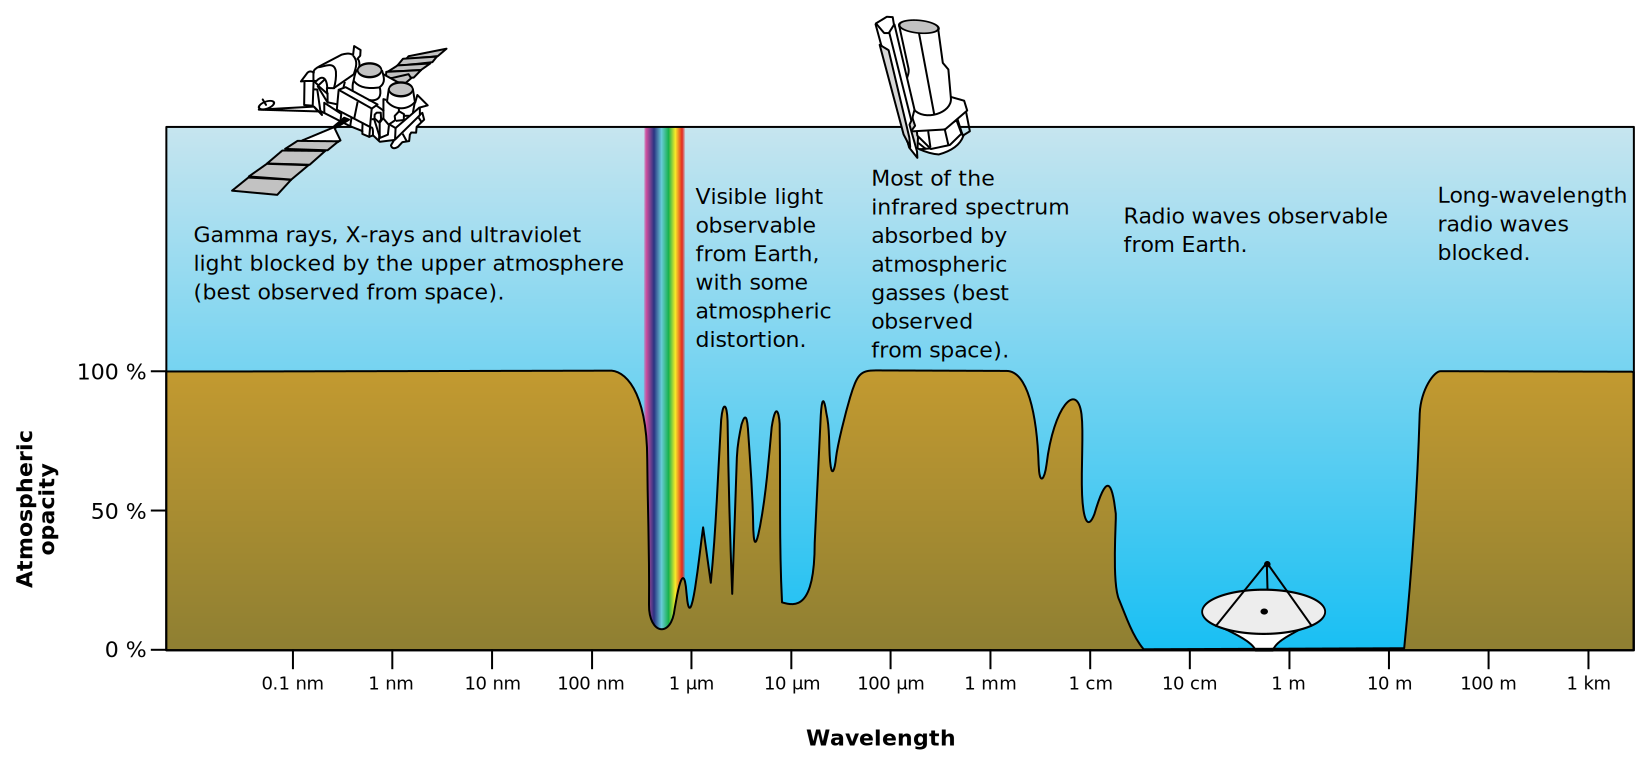
\includegraphics[width=\textwidth]{images/Atmospheric_electromagnetic_opacity}
\caption{Opacity of the Earth's atmosphere given different wavelength coming from space. Source \texttt{wikipedia}}
\label{fig:atmospheric-opacity}
\end{figure}

\begin{figure}[]
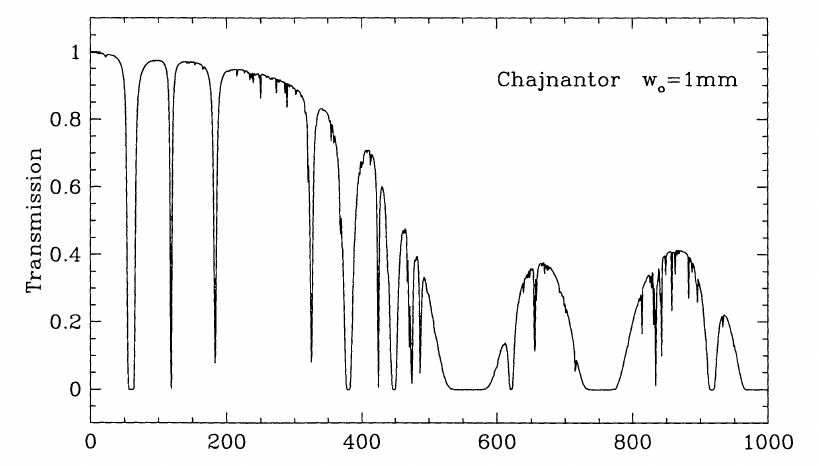
\includegraphics[width=\textwidth]{images/chajnantor-atm-transmission}
\caption{Transmission of the atmosphere from 0 to 1000 GHz for the ALMA site at Chajnantor in Chile assuming the typical value of $w_0 = 1 mm$ of precipitate water vapor. Source: \cite{taylor99}}
\label{fig:chaj-atm-tx}
\end{figure}

\begin{figure}[]
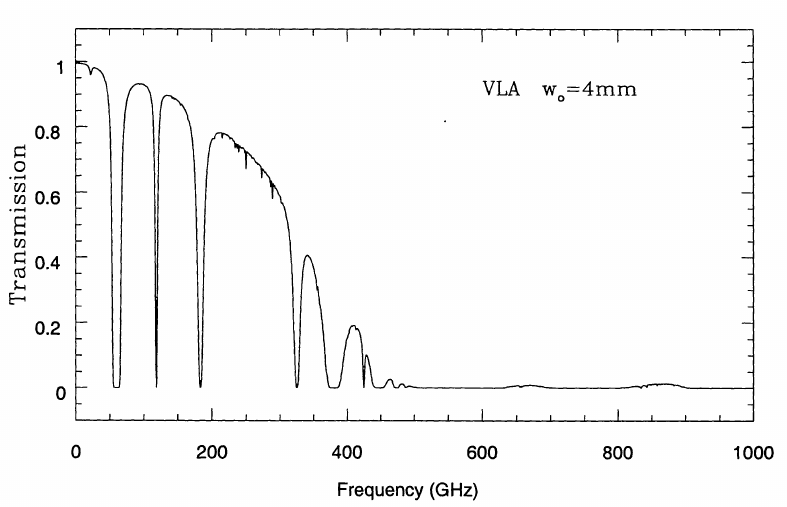
\includegraphics[width=\textwidth]{images/vla-atm-transmission}
\caption{Transmission of the atmosphere for VLA site in Socorro, NM, assuming a value of $w_0 = 4 mm$. Source: \cite{taylor99}}
\label{fig:vla-atm-tx}
\end{figure}

Figure \ref{fig:vla-atm-tx} shows the model of the atmospheric transmission at cm and mm wavelengths for the VLA site at 2150 m of altitude, figure \ref{fig:chaj-atm-tx} shows the model for ALMA site located in Chile at 4600 m of altitude. In both plots is possible to see a strong absorption lines including the water line at 22 GHz and 183 GHz, and the $O_2$ lines at 60 GHz and 118 GHz, plus a systematic decrease in the transmission with increasing frequency between lines. Every plot includes a different value for the column density of precipitable water vapor $w_0$ where each of one is typical for the site where the samples were taken. The precipitable water vapor (PWV) is the depth of the water vapor in the atmosphere in the site if it were converted to liquid phase.

Another important parameter in radio astronomy is the \textit{System Temperature ($T_{sys}$)}, this quantity measures the overall sensitivity of the receiving system. At centimetre, millimetre wavelengths, the temperature of the receiving system dominates the system noise temperature that is the receiver and the antenna. 

The calculation of $Tsys$ will be done in three steps:
\begin{enumerate}
\item First the Precipitable Water Vapor (PWV) content is determined. There are
several ways of doing this:
\begin{enumerate}
\item Calculate PWV from the Relative Humidity (RH) or the Dew Point. One way
of doing this is found in the MMA Memo No. 237, ``Precipitable Water at the VLA --
1990-1998'', by Bryan Butler. In this paper the PWV is developed as
$$
h = \frac{m_w P_0 H}{\rho_l k T_0}
$$
where $m_w$ is the mass of a water molecule (18 amu), $P_0$ is the water vapor
partial pressure, $H$ is the scale height of water vapor distribution (an
exponential distribution, 1.5 km for the VLA), $\rho_l$ is the density of
liquid water ($\mathrm{gr}/\mathrm{cm}^3$) and $k$ is the Boltzmann constant.

This memo presents a way to estimate $P_0$ from the dew point. In the subsequent
MMA Memo No. 238, ``Precipitable Water at KP -- 1993-1998'', a way of calculating
$P_0$ from the relative humidity is given:
$$
P_0 = 2.409 \times 10^{12} \ RH\ \theta^4 \exp(-22.67\theta)
$$
where $\theta$ is the inverse temperature ($\theta = 300/T_0 $ K), and $RH$ is
the relative humidity.

\item Calculate it from the opacity $\tau_{225}$ at 225 GHz measured by the
tipper. In this case a way of calculating the $PWV$ can be seen in
ALMA Memo 271 ``The Determination of Precipitable Water Vapour at Llano de
Chajnantor from Observations of the 183 GHz Water Line''. $PWV$ can be obtained
by inverting
$$
\tau_{225} = 6.7787\cdot 10^{-3} + 4.0757\cdot 10^{-2} PWV + 9.59\cdot 10^{-4} PVW^2
$$
\item Get the PWV directly from the Water Vapor Radiometers.
\end{enumerate}
When the $PWV$ is available from different sources, the different values
are averaged.

\item Interpolate the ATM tables to determine the opacity $\tau$ and the
atmospheric effective temperature $T_{atm}$. The ATM tables have the following structure:
\begin{eqnarray*}
\tau & = & \tau(\nu_i, PWV_j) \\
T_{atm} & = & T_{atm}(\nu_i, PWV_j)
\end{eqnarray*}
where $\nu_i$ covers the range $20-1000$ GHz with 100 MHz granularity, and $PWV_j$
covers the 7 values 0.4772, 0.658, 0.9134, 1.262, 1.796, 2.748, and 5.186 (mm). 
\item The system temperature is calculated as:

$$
T_{sys} = \frac {\left ( T_{rx} + T_{ant} + \xi T_{ant} \right ) e^{\tau / \sin(el)}}
{\eta}
$$
where $T_{rx}$ is the receiver temperature, $\eta$ is the forward efficiency (or
feed efficiency, or spillover factor), $T_{ant}$ is the antenna temperature and $\xi$
is the sideband ratio, which for practical purposes will be $0$

Expanding the calculation of above:

$$
T_{sys} = \frac{\left ( T_{rx} + \eta T_{atm} \left ( 1 - e^{-\tau/\sin(el)} \right ) + (1 - \eta) 0.95 T_{amb} + \eta 2.76 e^{-\tau/\sin(el)} \right )  e^{\tau / \sin(el)}}
{\eta}
$$
where $T_{amb}$ is the ambient temperature, which is read from weather station.
\end{enumerate}


\section{ALMA Project Data Model}
\label{sec:apdm}
The ALMA Software system works using the concept of an Observing Project, the full description and the details of the model are available at~\cite{apdm-model}. The Observing Project is used throughout the ALMA software as the top level structure associated with a project resulting from a single observing proposal. In fact the Observing Project is a container for all the information relating to a project before it begins execution. During and following execution other data associated with the project are created and held in other structures, each of which holds a reference to the original observing project. Of particular interest is the Project Status structure, which holds a record of the execution status of the Project. The ALMA Project Data Model (APDM) defines the structure of both the Observing Project (ObsProject) and the execution status (ProjectStatus).

The Scheduling Block (SchedBlock or SB) is the atomic unit of observing for ALMA, any given science observation will usually be broken into many SBs, which may, or may not be executed in sequence. The ALMA Scheduling Software will decide on which SB to execute at any given time on the basis of which is the best to execute now. An SB as a canonical execution length of around 30 minutes, however in practice the SBs observation duration could be up to 2 hours, depending of the Observation program.

\begin{description}
\item[Observation Project Entity] \hfill \\
When a ALMA user submits a project to the Data Base, then the user is creating a ObsProject. Almost all the end-user tools in ALMA operates on ObsProjects, no other entities are exposed to the end user.

In order to hold all of the pre-observing information associated with a project the ObsProject entity class is composed of three parts: an ObsProposal, an ObsReview and an ObsProgram. These hold the information associated with the three phases of observing preparation: the proposal or Phase I, the reviewing and resultant approvals, and the observing program definition, or Phase II.

\item[Observation Program Entity] \hfill \\
The Observing Program (ObsProgram) part of the Observing Project holds all the information created during Phase II, or program preparation. The ObsProgram consists of an Observing Plan (ObsPlan) and a SciencePlan. The Science Plan covers the science goal oriented view of the observing, and it is intended to contain the information that most users will use to define their observing programs. This information will persist, for the convenience of users, but will not be the definition that is used by the Observatory when carrying out the observations. Instead the latter information is contained within the ObsPlan, and covers what we call the system view. The service of Program Generation allows users to create the Observing Plan from their Science Plan. It is also possible for very advanced users to ignore the Science Plan and simply create all of the Observing Plan directly.

As stated, the Observing Plan (ObsPlan) is the container for defining the actual observing objects. In modeling terms the ObsPlan is a role for the top level ObsUnitSet, heading the definition of the system view. An ObsUnitSet contains a collection of Scheduling Blocks or more ObsUnitSets, along with objects defining the preconditions, performance and calibration requirements, and flow control that apply to that collection.


\item[Scheduling Block Entity] \hfill \\
A Scheduling Block (SB) is the unit of observing for ALMA. It defines all the information that is required by the Observatory to independently execute the acquisition of a set of data and then to calibrate it as well. Since SBs are selected for execution individually they must exist as separate items in the data base.

Most of the structures within the SB hold information that is used either by the scheduler, to query whether or not this SB is suitable for scheduling ``now'', or as information that is used by the Observing Script (in the Control subsystem) to actually execute the observing (see below), and in some cases both. There are also performance goals for the SBs, to be measured against by the observing system.

So to allow the determination of ``Schedulability'' we find items like representative target observability, weather constraints, a precondition that requires a current Baseline Calibration and a Scientific Priority.

\item[Targets] \hfill \\
The target is the element within an SB that defines the area to map, the spectral or instrumental setups to use, and the purpose of the observing. In fact the target element itself contains nothing except references to other elements that contain descriptions of these three key components.

\end{description}

\section{General problem}
\newtheorem{problem-def}{Definition}
The atomic unit to be scheduled is called scheduling block, this name matches the name described in section~\ref{sec:apdm}, although it differs since, the scheduling block is defined as atomic unit here, it contains only one target, the \textit{representative target}, which is the most representative of the set of targets for the given scheduling block. The submitter of the proposal is in charge to choose the representative target.


\begin{problem-def}
A Scheduling Block (SB) is represented as a n-tuple of time independent  properties ($P$). Let $S_0$ be the set of all SBs,
$$S_0 = P_1 \times P_2 \times ... \times P_n,$$
for appropriate $P_i$ sets. Then one SB is:
$$sb = (p_1, p_2, ..., p_n) \mid p_i \in P_i$$
\end{problem-def} 

Once defined a scheduling block, then the operation of selecting SB can be defined as:
\begin{problem-def}
The scheduling blocks selection is represented as a function that for a given time $t$ and a set of SBs $S \subseteq S_0$, it returns a subset of S:
$$sel:(t,S) \rightarrow \mathcal P \left({S}\right)$$
\end{problem-def}

Given these definitions, a property of $sel$ follow:

\newtheorem{sel-props}{Property}
\begin{sel-props}
The full selection operation $sel$ for a given time $t$ can be decomposed in independent selection operations, one for each property $p_i$:
$$sel(t,S) = sel_1(t, S) \cap sel_2(t, S) \cap ... \cap sel_n(t,S)$$
In general, each one of these selection operations can be expressed  as an inequality, defining the ``schedulable time window'' for a given $sb_j$:
$$sb_j \in sel_i(t, S)\,i.i.f\;\alpha_1(t, sb) \leq \alpha(t, sb) \leq \alpha_2(t, sb)$$
\end{sel-props}

Without losing generality, the inequality of the property of above can be separated in two inequalities, then the condition can be expressed as: 
$$\alpha'(t, sb) \leq \alpha (t, sb)$$
Regarding the dependencies of both $\alpha$ and $\alpha'$, if the property depends on $t$, then the property is \textit{dynamic}, which means that the property value to satisfy the inequality is calculated and updated accordingly the scheduling algorithm progress. In other hand the properties depending only on $sb$ are \textit{static}, therefore the values to satisfy their inequalities are pre-calculated at the beginning of the algorithm.\\

\subsection{Static an dynamic constraints}

As stated in section~\ref{sec:apdm} a target is composed by three elements, which match the constraint categories detailed here: \textit{sky source}, \textit{instrumentation} and \textit{weather}.

In common terms a Scheduling Block is ``schedulable'' only if the representative target for the given scheduling block is observable, this means that the source of the sky is visible, the array configuration has enough hardware capabilities to observe the source according to the scientific plan, the weather conditions are good enough to carry on the observation, etc. Basically this is the intersection of the different $sel$ functions and it is defined as the \textit{schedulable time window} for a given scheduling block, this window could be available several times during the observing season. In practical terms a scheduling block can be observed as many times as possible until it has been complete.

The description of each one of the different categories is as follow:

\begin{description}
    \item[Instrumentation] \hfill \\
Every scheduling block execution is done in an \textit{Array} which is a subset of the available antennas in the observatory. Each antenna has its own hardware configuration to receive electromagnetic waves from the space. An array will have the hardware configuration common to all the antennas conforming the array, the idea is to observe the target with the same hardware in all the antennas as they were a single instrument. In general, in an observatory all the antennas conforming an array will have all the same capabilities, even they can be interchange each other and should not be any difference. The array configuration and the availability of the instrumentation is decided beforehand and for effects of the algorithm is considered an static constraint. 

Nonetheless, problems in some instruments during observatory operations could temporally remove some capabilities from some antennas, or even the entire antenna could be removed, altering the original instrumentation properties that the array was given initially. Since all these failure are not planned this is considered a dynamic constraint.

	\item[Sky source] \hfill \\
In general a sky source will be visible in daily basis for certain amount of time, then the source will go below horizon due the Earth's rotation, unless the source is circumpolar in which case the source will be always visible. Also the Earth's orbit movement around the sun would cause that a source will be visible during a period of the calendar year only. Both of these source properties are predictable and can be calculated before the execution of any observation.

Every time that a observation starts, the telescope needs to be calibrated to adjust pointing corrections based on atmospheric conditions and source position. It is possible to predict how much time will be spent on calibrations if the observation plan is given before the execution of observations starts, however sometimes this is not the case due improvement or deterioration of weather conditions expected, making this constraint dependable on the time the observation being executed.
  
	\item[Weather] \hfill \\
The weather cannot be foreseen with exactitude, even the most accurate weather forecast will have a error margin, which will increase if the period of time foresaw increase. Once the weather condition has changed, for good or bad, usually the list of the scheduling blocks to be observed needs to be updated accordingly. The time frame on what the algorithm can optimize the observations is bounded to the reliability of the weather pattern prediction, doing optimizations beyond that could be worthless.

\end{description}

Another important property of every project submitted to be observed in the observing season, is that they does not have the same science value, this means there are certain projects that are more interesting to observe and complete than others. This measure of how much value has a project is given by science team of the observatory, therefore the scheduler must be aware of this and try to complete most of the projects having the ``highest'' science qualification, this will be known as the \textit{scientific throughput}.

\subsection{Completing Scheduling Blocks and Observation projects}
\label{subsec:completing-obs}
A scheduling block does not need to be completed in just one observation, in fact the scheduling block cn be observed multiples times at different time, hence different weather conditions and different array configurations, until the scheduling block is considered complete.
A scheduling block will be completed, and put its state as complete, if it meets any of following three criterion:
\begin{itemize}
	\item \textit{Number of repetitions}: A scheduling block could have a limit of how many times can be observed.
	\item \textit{Total time observed}: A scheduling block could have a limit of how much time can be observed.
	\item \textit{Sensitivity achieved}: As stated in section \ref{sec:sens} if the goal for the RMS noise accumulated is achieved, then the scheduling block will be considered completed.
\end{itemize} 
Some of the scheduling blocks could not have all the three criteria, it is enough for the SB to have a least one of them.

The criteria to determine if a project was complete, is based in how many scheduling blocks or ObsUnit sets have been completed, or the total amount of time observed, which is the sum of all the scheduling blocks observations. However, in reality human intervention is required to determine if the project has been completed based on the quality of science data extracted from the observations. The algorithm establishing whether a Observation project is completed or not is far beyond the scope of this study. 

\subsection{Observing season (Observation cycle)}
Until this point, this study has tried to explain and referred only to observation properties within the time frame considering only one instrument (just one instrument spawns for the whole observation time frame). 

However, over the whole time available in the observing season, it is possible to have different \textit{Array configurations}, that can co-exist at the very same time with other array configurations, or can be created in serial over the time frame of the observation season, or a combination of both situations.

Each array configuration can be composed of 1 or more antennas available at the observatory, each one can offer different science capabilities, which can be or cannot be used by the scheduling block, nonetheless each array will offer basic differences like the $uv$ coverage as seen in section \ref{sec:uvcover}, the angular resolution explained in section \ref{sec:angular-res} or the sensitivity achieved in every observation (section \ref{sec:sens}), which is dependent of the number of antennas in the array. As well one or more arrays can be available for observations at the same time as said before, however each scheduling block must be observed by just one array at a given time.

\subsection{Identified problems}
\label{sec:problems}
After the analysis of the different properties and constraints related to the astronomy scheduling problem it is possible to identify the following two different problems:
\begin{description}

\item[Scheduling array problem] \hfill \\
The \textit{scheduling array problem} consists on determine a schedule for a given set of scheduling blocks, which all of them can be observed by the instrument, considering one array already created within a given period of time. 
The idea is to generate a plan to try to observe all, or most of the projects with the highest scientific value in the less amount of time possible considering all, or the most critical of the scientific requirements. It may possible to not complete all the observation projects submitted for this array configuration. Slso is desirable to reduce the amount of idle time of the instrument.

\item[Array configuration schedule problem]

The \textit{array configuration schedule problem} is on top of the scheduling array problem. It consists in try to determine a schedule of observations, for the observing season (which is a fixed amount of time and it lasts for several months, up to a couple of years), for a given set of the scheduling blocks and a given set the array configurations. The idea is to try to observe most of the projects with high scientific value considering all, or most of the scientific requirements during the observing season, however not all the observation projects may not be completed. Also it is desirable to reduce the idle time of the observatory as whole.
\end{description}


\section{ALMA Scheduling Problem}
\label{sec:alma-sched-problem}
The Atacama Large Millimeter/submillimeter Array (ALMA) is a major collaboration effort between European, North American and East Asian countries, under construction on the Chilean Chajnantor plateau, at 5.000 meters altitude. When completed in 2013 it will be the largest radio telescope on earth, with more than 60 antennas of 12 and 7 meters diameter, distributed over a wide extension, with up to 16 kilo-meters of baseline separation. The ALMA interferometer will provide the possibility to be used as a single array, or as up to six (due to limited centralized equipment, photonic references) minor independent arrays or groups of antennas. As each array is equivalent to one instrument, this can eventually be seen as a multi-telescope problem. Also, the antennas will be changing their positions over the year, as different distributions will be used to exploit various kinds of observations. As ALMA does not observe in the visible spectrum, observations are not limited to night time only, thus a 24/7 operation with as small downtime as possible is expected. 

ALMA will operate exclusively in service mode. Therefore, the Scheduling software Subsystem is supposed to provide a fully automatic “quasi-real-time” dynamic scheduling platform, mostly with the only human participation of supervision. This Subsystem is still under development, and the needed algorithm(s) are still in a preliminary state. The main problem is the dynamic priorities scheduling, which differs widely from the traditional dynamic job-shop. This particular problem is very similar for all ground based observatories, and ALMA is one real example, that needs this kind of scheduling to accomplish its operations requirements.

The ALMA telescope will be operated as one or more antenna arrays, executing observation blocks corresponding to accepted project proposals. There will be three different antenna types, provided by three vendors:
\begin{itemize}
\item 12-m antennas (50): This is the main array to be operated, and also the one to be divided into several sub-arrays. They are provided by vendors Vertex (Vertex Antennatechnik GmbH) and AEM (Alcatel Alenia Space France, Alcatel Alenia Space Italy, European Industrial Engineering S.r.L., MT Aerospace).

\item 7-m antennas (12): This is the main part of the ALMA Compact Array (ACA), which will  operate as a separate array. They are provided by MElCo (Mitsubishi Electric Corporation).

\item 12-m total power antennas (4): These are special total power antennas able to see a full 2GHz spectrum, part of the ACA, but in principle exchangeable with any of the other 12-m antennas. They are also delivered by MElCo.

\end{itemize}

\begin{figure}	
\begin{center}
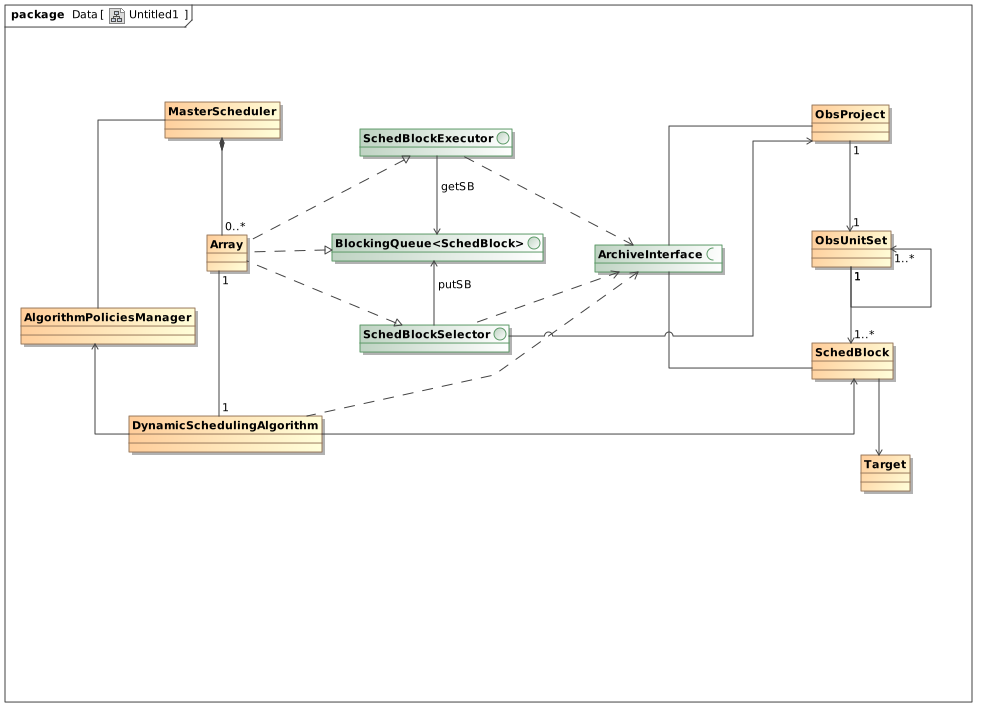
\includegraphics[width=\textwidth]{images/scheduling_class_model}
\caption{Basic class model of Scheduling subsystem.}
\end{center}
 \texttt{MasterScheduler} and \texttt{Array} are the common classes used by all kind of Arrays. \texttt{DynamicSchedulingAlgorithm} is the class implemenenting the current ALMA's dynamic algorithm. At right side of the figure it is available the hierarchy of the the top level APDM classes used by the scheduling subsystem, which are accessed through the \texttt{ArchiveInterface}.
\label{fig:sched-class-model}
\end{figure}

A huge part of the telescope operations will be handled through the ALMA software, which is divided into various subsystems, such as Control, Correlator (ACA and Baseline), Pipeline, Archive, Scheduling and Offline software. The big picture of ALMA Software can be seen in~\cite{schwarz04}.
The Scheduling Subsystem is the one in charge of managing antenna arrays and dynamically executing scheduling blocks. The current software design details are in~\cite{clarke12}. The basic design considers 4 main parts which are represented in figure \ref{fig:sched-class-model}: The ``Master Scheduler'', The ``Array'', The ``Dynamic Scheduler instance'' and the ``Archive Interface''. The Master Scheduler is in charge of create and manage the creation of the Arrays and handle the management of the Scheduling Policies to be used in the DSA. The Array is the main operations unit of the scheduling subsystem, each array operates over Scheduling Blocks, executing, waiting for results of the observations and notifying to the user of the system what has been the outcome of the observation. The Array uses directly the Archive, which is the database storing the definition of each Observation project (see~\ref{sec:apdm}), through the Archive Interface. Each array has its own scheduling queue, which can contain several schedblocks waiting to be executed, but just one SchedBlock is observed at the same time in each Array. Finally the DSA acts as a component of an Array selecting the current best SB according to the algorithm policy selected for the given Array, the details of the ALMA's DSA is discussed in section \ref{sec:alma-dsa}. Additionally each scheduling array can operate in 3 different modes: Manual, in this mode the scheduling queue is set with a maximum of one item, in this mode the user is responsible to execute the observation manually using low level scripts. Automatic, in this mode the array has a unlimited size scheduling queue, once a observation has been completed a new SchedBlock is taken from this queue to observe the next one until the queue is empty or the scheduler is stopped. And Dynamic, in dynamic mode the scheduling queue behaves as the array in interactive mode, but when the queue is empty the DSA is triggered selecting the next best SchedBlock to observe, depending if the DSA is active or passive the selected SchedBlock will be put in the queue to start the observation or the Scheduler will notify the user only respectively. The state machine implemented as part of the current DSA can be seen in the figure~\ref{fig:sched-dsa-state-machine}, the DSA may be executed every time that a new Scheduling Block is needed to be queued, until there is no more Scheduling Blocks available.

\begin{figure}	
\begin{center}
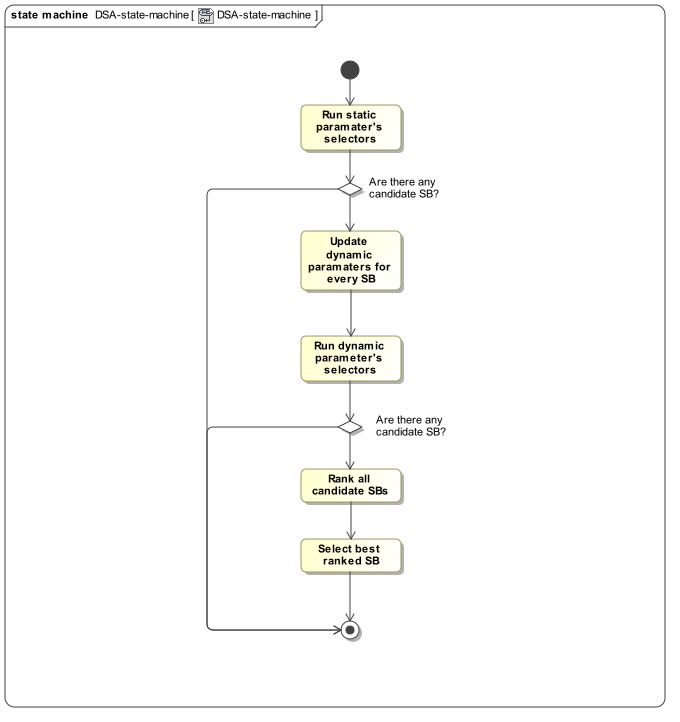
\includegraphics[width=0.9\textwidth]{images/DSA-state-machine}
\caption{Dynamic scheduling algorithm's state machine}
\end{center}
\label{fig:sched-dsa-state-machine}
\end{figure}


It is true that most of the scheduling software will be run in the on-line software, however there is a planning stage where the Scheduling algorithm will contribute to plan different scenarios within a season. The on-line usage of the algorithm is known as the \textit{short-term scheduler}, this scheduler either can be used in quasi-real time or to planning the night observations. A \textit{medium-term scheduler} used to planning the observations for a time frame where the array configurations are the same. And finally \textit{long-term scheduler} which should be able to plan an entire season of observation across the different array configurations, ideally the algorithm should define the duration of each configuration given as a input. For the two last use cases a ALMA scientific operations uses a simulator, which is mostly described in~\cite{hoffstadt10}. Although new features have been added, the basic workflow has been kept until nowadays.
\chapter{Proposed Solution}

As stated in section~\ref{sec:problems} two problems were identified, these both problems are part of the ALMA Scheduling problem.
This chapter describes the proposed solution for both problems, which are related between each other.
The solution is modeled after ALMA requirements and current software design detailed in~\cite{avarias11,clarke12,schwarz04,apdm-model} and it aims to solve the ALMA scheduling problem. Although some simplifications are considered, mainly because still there are certain requirements that are under discussion or they are still unclear. 

\section{General conditions and simplifications}

As stated in~\ref{sec:alma-sched-problem}, each array is handled independently by the scheduling subsystem software, this means that each array will have its own scheduler instance, and they are considered a different instrument during them life. At very same time one or more arrays can be running, hence the multiple schedulers instances can be active, and the data containing the Observation Projects and Scheduling Blocks is common to all the schedulers.

Even though is possible to have linked Scheduling Blocks between each other, the solution proposed here will not considered here due they are not well defined in the ALMA requirements and they are still in discussion. This implies that the Scheduling Blocks belonging to an Observation Projects can be observed and completed in any order.

Instrument calibrations and pointing is a very important step before the actual usage of the instrument, increasing the accuracy and sensitivity of the instruments. However, for now, the algorithm will consider that the array configurations are always calibrated and ready to observe. Also session management will not be considered at all due calibrations dependencies.

The time period to be scheduled could not be continuous, this means that there may be time periods during the day where the instruments will not function to produce science. Since this is planned, the time not used for science is not considered as downtime. Dynamic or random downtimes have been not considered and they are out of the scope of the problem.

The time spent in a single execution (observing) is variable, it depends completely on the Scheduling Block to be observed. Usually the requested duration goes from 30 minutes until 3 hours. The Observation project and Scheduling Blocks will be considered completely observed according to the rules discussed in section~\ref{subsec:completing-obs} 

The DSA will do the search based on the Local Sidereal Time (LST).

The arrays configurations are given as input to the algorithm, the algorithm will try to accommodate over the time the given configurations. It is not responsibility of the algorithm to come up with suggestions related to changes in the configurations.
 
\section{ALMA Scheduling array problem}

This problem only considers the execution of Scheduling Block inside the same Array Configuration. The algorithm lifecycle is tied to the current ALMA requirements shown in section~\ref{sec:alma-sched-problem} figure~\ref{fig:sched-dsa-state-machine}, which is detailed as follows:

\begin{description}
\item[Run static parameter's selector] \hfill \\
After running these selectors the algorithm will return a list of the potential candidates given current static conditions, this includes the visibility for the representative target which is known beforehand, but is not filterable until the algorithm knows the current Local Sidereal Time. If after this state there is no feasible solution, then the algorithm will return nothing.

\item[Update dynamic parameters] \hfill \\
In this state the algorithm will recalculate the parameters requiring update at the given time. Usually weather conditions and parameters that cannot be calculated beforehand (e.g. altitude of a source for the given time, the point in the sky is in RA-Dec coordinates).  

\item[Run dynamic parameter's selector] \hfill \\
This will filter out all the Scheduling Blocks which do not fit in the criteria established after the dynamic updates ran. As the first state it will return a list of the candidate SB. If after this state there is no feasible solution, then the algorithm will return nothing.

\item[Rank all candidate Scheduling Blocks] \hfill \\
The algorithm might have a list of scorers, each one of these ``scorers'' will assign a value between ${[ 0 , 1 ]}$. The algorithm also will have a list of weights, one per scorer. The final result of each Scheduling Blocks will be sum of all the weighted scores given to this Scheduling Block for the given time to the algorithm.

\item[Select best ranked Scheduling Block] \hfill \\
The algorithm will select, and will return, the ``best'' suitable Scheduling Blocks for the given time.

\end{description}


\subsection{Mathematical model}
\label{sec:array-sched-math-model}

\subsubsection{Static parameters}
These parameters are statically provided at the beginning of the period. They do not change over the time period being used by the algorithm.

\begin{description}
\item[$\mathbf{P_i}$] Project number $i$ $\Big\slash \forall P_i \mid P_i \neq \emptyset \land P_i = \{SB_{i1}, SB_{i2}, \ldots, SB_{ik}\}$.

\item[$\mathbf{SB_{ik}}$] Scheduling Block $k$ $\Big\slash \forall SB_{ik} | SB_{ik} \in P_i \land SB_{ik} \notin P_x \Leftrightarrow x \neq i$.

\item[$\mathbf{SciVal(P_i)}$] Scientific value for $P_i$ $\Big\slash \forall P_i \land SB_{ik} \in P_i \mid SciVal(P_i) \Leftrightarrow SciVal(SB_{ij}) $.

\item[$\mathbf{T(SB_{ik})}$] Duration (time) of a single execution (observation) for Scheduling Block $ik$.

\item[$\mathbf{AC_j}$] Array Configuration $j$.

\item[$\mathbf{T(AC_j)}$] Duration (time) for Array Configuration $j$.

\item[$\mathbf{Type(AC_j)}$] Type of Array Configuration number $i$ $\Big\slash Type(AC_j) \in \{12m, 7m, TP\}$.

\item[$\mathbf{Ex_h}$] Executive number $h$.

\item[$\mathbf{TP(Ex_h)}$] Percentage of time for Executive $h$ $\Big\slash \forall TP(Ex_h) \mid TP(Ex_h) \in {[0,1]} \land \sum_{h}^{n} TP(Ex_h) = 1$ 

\end{description} 

\subsubsection{Dynamic parameters}
Contrary to the static parameters, these parameters may change at any time during the time period being used by the algorithm.

\begin{description}
\item[$\mathbf{EB_n}$] Execution Block $n$. The execution blocks represents a time frame where an observation of Scheduling Block $SB_{ij}$ was carried on, it belongs to a given array configuration $AC_j $, since start time $t_s(EB_n)$ until end time $t_e(EB_n)$, during this period of time and array configuration the execution block is unique.

\item[$\mathbf{T(EB_n)}$] Duration (time) of Execution Block $n$.

\item[$\mathbf{LST}$] Current Local Sidereal Time.

\item[$\mathbf{St(P_i)}$] Current status of Project $i$  $
\left\{
\begin{array}{l l} 
true & \mbox{if  } P_i \mbox{ completed} \Leftrightarrow \forall SB_{ik} \in P_i \mid St(SB_{ik}) = true\\
false & \mbox{if  } P_i \mbox{ not completed} \\
\end{array}
\right .$

\item[$\mathbf{St(SB_{ik})}$] Current status of Scheduling Block $ik$  $
\left\{
\begin{array}{l l} 
true & \mbox{if  } SB_{ik} \mbox{ completed} \\
false & \mbox{if  } SB_{ik} \mbox{ not completed} \\
\end{array}
\right .$

\item[$\mathbf{\tau_{225}(SB_{ik}, t)}$] Opacity for a given Scheduling Block's source $ik$, for the given time $t$.

\item[$\mathbf{T_{sys}(SB_{ik}, t)}$] System temperature for a given Scheduling Block's source $ik$, for the given time $t$.

\end{description}

\subsubsection{Objective functions}

The main objective of the algorithm is to maximize the number of scientific projects completed at the end of the time frame given. Also it can be interpreted as to maximize the scientific value of the completed projects (see equation~\ref{eq:max-sci-value}). However there is a caveat, there must be priority on complete the best graded projects.

\begin{equation}
\label{eq:max-sci-value}
max \: \bigg(\sum_{i} SciVal(P_i) \times St(P_i)\bigg)
\end{equation}

At the same time the algorithm, must maximize the array's usage time. This is equivalent to minimize the array's idle time (see equation~\ref{eq:min-idle-time}).

\begin{equation}
\label{eq:min-idle-time}
max \mbox{ }\Bigg( \frac{\sum_{i}T(EB_i)}{T(AC_j)}\Bigg)
\end{equation}


\subsubsection{Constraints}
\label{sec:sched-constraints}
It is assumed that all the constraints operate over one or more Scheduling Block's properties, unless stated.

\begin{description}

\item[Executive time balance] \hfil \\
ALMA observatory is based on international collaboration. Within this collaboration several countries participate through science and astronomical organizations. Currently these organization are divided among different world's regions, which are called executives. These executives are North America (NA), Europe (EU), East Asia (EA), Chile (CL) and Non Alma members (OTHER).

Since each executive contributed with different resources, which may differ from the other executives. A fixed percentage of the total observation time of a observation cycle is given to each executive. Ideally, the assigned amount of observation time shall be adjusted to comply with the percentage assigned to each executive.

Ideally, the observation time percentage for each executive, has to be kept accordingly to the assigned percentage in the observation cycle. Nonetheless, this could carry unfairness within each observation sub-period (e.g within one week only NA Scheduling blocks were observed). This could trigger unhappiness and some concerns among the different executives, whom expects to have their observation time proportion assigned during a sub-period of time within the observation cycle.

It has been defined the period of time, as one week of observation (this coincides with the early science block carried on bi-weekly). Within this period of time each executive shall get as near as possible the amount of time assigned initially. If it is not possible, then the scheduler shall carry over the unfairness among the executive's times and apply corrections in future schedules (see equation~\ref{eq:exec-balance}).

\begin{equation}
\label{eq:exec-balance}
\frac{\sum_{i}^{n} T(EB_x)}{(t_e - t_s)} \approx TP(Ex_j) \mid  EB_i \in Ex_h \land t_s \leq t_s(EB_i) \land t_e(EB_n) \leq t_e
\end{equation}

Where $T(EB_x)$ is the time observed for a given Execution Block $EBxi$, $Ex_h$ is a given Executive; and $t_s$ and $t_e$ are the starting and ending times for a arbitrary time interval, as expressed before for convenience, this time interval may correspond to a single week of observations.

At the end of the cycle is expected that each Executive will receive the time assigned to it or a very near value. 

This constraint is a special kind, since it operates over a set of Execution Blocks after the observation of one or more Scheduling Blocks, over a period of time. Instead of operate over a Scheduling Block property.

\item[Right Array Type]
ALMA observatory will have several types of arrays. The algorithm must not choose the Scheduling Blocks which are not possible to observe on the current Array Type (equation~\ref{eq:array-type-sb}).

\begin{equation}
\label{eq:array-type-sb}
Type(AC_j) = Type(SB_{ik})
\end{equation}


\item[Source visibility] \hfill \\
It is possible to know before running the algorithm, to know if a point in the sky will be visible at the time when the algorithm runs.
In function of $LST$ the rising and setting, $LST_r$ and $LST_s$ shown by equation~\ref{eq:lst-r} and equation~\ref{eq:lst-s} respectively.
\begin{equation}
\label{eq:lst-r}
LST_r =  24 - \frac{1}{15} \cos^{-1} (-\tan\phi\tan\delta) + \alpha
\end{equation}
\begin{equation}
\label{eq:lst-s}
LST_s = \frac{1}{15} \cos^{-1} (-\tan\phi \tan\delta) + \alpha
\end{equation}

Also is possible to known if the source is always visible or hidden as shown in equation~\ref{eq:sky-src-always-vis} and~\ref{eq:sky-src-always-hid} respectively.

\begin{equation}
\label{eq:sky-src-always-vis}
visible \Leftrightarrow
\left\{
	\begin{array} {l l}
	\delta > (90^\circ - \phi) & \mbox{ for northern hemisphere} \\
	\delta < -(90^\circ + \phi) & \mbox{ for southern hemisphere} \\
	\end{array} 
\right.
\end{equation}
\begin{equation}
\label{eq:sky-src-always-hid}
hidden \Leftrightarrow
\left\{
	\begin{array} {l l}
	\delta < -(90^\circ - \phi) & \mbox{ for northern hemisphere} \\
	\delta > (90^\circ + \phi) & \mbox{ for southern hemisphere} \\
	\end{array} 
\right.
\end{equation}

where $\alpha$ is the right ascension, $\delta$ is the declination, and
$\phi$ is the telescope geographical latitude.


The selection operation selects all the SBs for which the current $LST$ falls
between $LST_r$ and $LST_s$, accounting for cases where this range extends to include
the following day (see equation~\ref{eq:lst-range-sel}).

\begin{equation}
\label{eq:lst-range-sel}
S(LST) = \left\{ 
	\begin{array}{l l}
	LST_r < LST < LST_s & \mbox{if } LST_r < LST_s \\
	LST_r < LST < 24 \land 0 \leq LST < LST_s & \mbox{if } LST_r > LST_s  \\
	true & \mbox{if } src(SB_{ik}) \mbox{ is always visible.} \\
	false & \mbox{if } src(SB_{ik}) \mbox{ is always hidden.} \\
	\end{array} \right .
\end{equation}

The $LST$ parameter is the current Local Sidereal Time, over what the algorithm is selecting Scheduling Blocks.

\item[Sun avoiding zone] \hfill \\

\item[Moon avoiding zone] \hfill \\

\item[Array configuration and resolution] \hfill \\
A first order approximation of the resolution that can be attained with a give
array configuration is $\theta = \lambda / l_{max}$ where $l_{max}$ is the maximum
baseline in the array. Each SB defines a range of acceptable resolutions $[\theta_{min}, \theta_{max}]$ (see equation~\ref{eq:sel-arr-res})
\begin{equation}
\label{eq:sel-arr-res}
\theta_{min} \leq \frac{\lambda}{l_{max}} \leq \theta_{max}
\end{equation}

\item[Atmospheric transmission] \hfill \\
For atmospheric transmission selection a simple criteria is used based in opacity quartiles at 225 GHz.

\begin{equation}
S(\nu_{rep}, \tau_{225}) = \left\{
    \begin{array}{l l}
    true & \mbox{if } \nu_{rep} > 370 \mbox{ GHz } \land \tau_{225} \leq 0.037 \\
    true & \mbox{if } 370 \mbox{ GHz } \geq \nu_{rep} > 270 \mbox{ GHz } \land \tau_{225} \leq 0.061 \\
    true & \mbox{if } \nu_{rep} < 270 \mbox{ GHz } \land \tau_{225} \leq 0.6\\
    false & \mbox{otherwhise}
    \end{array} \right . 
\end{equation}

where $\nu_{rep}$ is the representative frequency at $\tau_{225}$ is the Opacity
at Zenith at 225 Ghz.

\item[Weather stability] \hfill \\
During the execution of an observation, the algorithm must try to ensure that the weather conditions would not deteriorate significantly.
For this purpose, the $Tsys$ is calculated using an average of a few data
points taken at the time when the algorithm is executed, then this value is compared with the
projected $Tsys$ calculated at least 30 minutes later
%, taking also into consideration the change in elevation of the SB representative target.

How significant the increase in $Tsys$ needs to be for a SB to be discarded
is under discussion, and in general it will be frequency dependent. In addition
it is possible that some projects decide that non-optimum observing conditions are
fine anyway. For now, an increase in the $Tsys$  of 15-20\% is considered too much
degradation for the SB to be executed.

The selection operation filters out all the SBs that don't comply with equation~\ref{eq:sel-tsys}
\begin{equation}
\label{eq:sel-tsys}
\frac{T_{sys}(t+\Delta t) - T_{sys}(t)}{T_{sys}(t)} < 0.15
\end{equation}

\end{description}

\subsubsection{Algorithm design rationale}

So far, the study has been focused in the definition of the ALMA's Scheduling array problem and the study of its mathematical model. However, this have not provided the background about how the algorithm will operate internally to return a plan for a given time period. The decision of the algorithm design is driven by the following properties:
\begin{enumerate}
\item The algorithm must work on the on-line system and as well on simulation mode. The idea behind the simulation, is to evaluate how well (or bad) behave the algorithm for a given set of Scheduling Blocks, Array Configurations and time period. Since the ultimate goal is to use the algorithm in on-line system to contribute to take a decision for the best Scheduling Block at a given time.

\item The time within a time period, used by the algorithm, might not be discretized because of the variable duration of each Scheduling Block. Also a single execution of a Scheduling Block is not be preemptable until it completes (success ot failure). 

\item The algorithm must try to optimize the objective functions (equations~\ref{eq:max-sci-value} and~\ref{eq:min-idle-time}), but at the same time the executive percentage time balance must be kept in line, according to the original defined values, within an observation time frame of one (1) week (see equation~\ref{eq:exec-balance}).

\item The algorithm design and implementation must fit into lifecyle currently in use by ALMA software.

\end{enumerate}

Given the uncertain number of possible Execution Blocks, duration of them and the time when they are scheduled for execution, it might result impossible to determine a domain model where a complete search technique could be applied. Also, every time a Scheduling Block is scheduled for observation, the search tree for the problem changes, creating a whole new set of options based on the previous decision. Of course, the dynamism on the number of branches in the search tree, greatly depends on the number of Scheduling Block given as input for the algorithm. According to ALMA's system requirements the scheduling subsystem (including the algorithm) must be able to handle easily~\footnote{Easily is a quality property for the system, which should be interpreted as ``The algorithm must return a solution in a reasonable human time (usually between $1-2$ seconds)'' for the given input time} $10000$ Scheduling Blocks as input.

The algorithm proposed in this study will be based on the Deficit Round-Robin (DRR) algorithm~\cite{shreedhar96}. The original algorithm defines service flows (queues) and a processor dispatching the network packets arrived and already sorted in one of the flows. Making a comparative between the model proposed in the original paper and the ALMA's scheduling problem, it is possible to map the original proposed domain model into the ALMA's model as follows:

\begin{description}
\item[Network packets] are mapped into a \textit{single-execution of a Scheduling Block}. This is not the same as the Execution Block, because this entity is the result after a Scheduling Block execution. As established by DRR design, the network packet length is variable, matching the single-execution time Scheduling Block property.

\item[Processor] is mapped into the \textit{Array Configuration}. The Array is unique and can execute just one Scheduling Block at a given time.

\item[Service flows] are mapped into the \textit{Executives' observation times}. Actually, the flows will be mapped into the percentage of the Executives' observation times, what is a measurable quantity given an arbitrary time frame inside the total duration of the time given as input to the algorithm. Nevertheless, the mapping here does not fit perfectly, due the design of DRR establishes that every service flow will have the same priority than the others. For the ALMA case, each Executive should have different priorities, to deal with this issue a weight will be applied to the quantum size, based on the time percentage assigned to each executive, this is similar to what is proposed in the weighted Round-Robin algorithm explained in~\cite{katevenis91}.
\end{description}

In the original DRR algorithm, the service flows are filled with network packets arriving from the media, and they are kept in the queues until are services. In ALMA, each service flow will be filled with the result of the Scheduling Block filtering for the given time based on the mathematical model constraints explained in section~\ref{sec:array-sched-math-model}. The difference with DRR is that the service flows will be recalculated every time the algorithm runs, filtering-out and putting-in the no longer and new suitable Scheduling Blocks respectively.

The quantum size will be fixed number as explained in the original DRR design. However, the quantum size applied to a Executive's service flow will be multiplied by a weight defined in equation~\ref{eq:alg-quantum-weight}, which is different for every Executive.

\begin{equation}
\label{eq:alg-quantum-weight}
W_{h} = \frac{TP(Ex_h)}{max(TP(Ex_x))}
\end{equation}

To achieve the objective functions, the algorithm must optimize the selection for the given time. For this reason, the Scheduling Blocks must be prioritized according to a score. This score shall be composed by the sum of different weighted scores, very similar to what is proposed in the current ALMA algorithm. The following are the scorers currently defined for the current ALMA DSA, that can be reused for the proposed algorithm in this study:

\begin{description}
\item[Scientific priority score] \hfill \\
Each proposal or project gets assigned a scientific priority, defined by three numbers
(score, rank, grade). The \texttt{score} (a float) is assigned by
a specialized committee (galactic, extra-galactic, etc.). When the proposals that have
been evaluated by different committees are assembled in one set, there is the possibility
of collisions in the order defined by the \texttt{score}. The \texttt{rank} (an integer) resolves these
collisions, providing a completely ordered set. On top of this, the \texttt{grade} (which can assume
the values A, B, C, or D)

The algorithm computes the scientific priority score as shown in equation~\ref{eq:project-grade-score}
\begin{equation}
\label{eq:project-grade-score}
S = \frac{N_p - (\mathtt{rank} - 1)}{N_p} + K
\end{equation}
where $N_p$ is the total number of projects (or proposals), and $K$ is defined by equation~\ref{eq:scoring-prj-grades}
\begin{equation}
\label{eq:scoring-prj-grades}
K = \left\{
    \begin{array}{l l}
    4 & \mbox{if project grade is $A$} \\
    2 & \mbox{if project grade is $B$} \\
    1 & \mbox{if project grade is $C$} \\
    0 & \mbox{if project grade is $D$}
    \end{array} \right . 
\end{equation}

\item[Hour angle score] \hfill \\
In order to favor the Scheduling Blocks that at the current time have their representative source close to the zenith, 
their hour angle should be in the vicinity of $0.0$ hours. The hour angle score is defined in equation~\ref{eq:ha-scorer}

\begin{equation}
\label{eq:ha-scorer}
	S = \frac{AM_{current}}{AM_{transit}} = \frac{\cos(HA) + \tan(\delta) \tan(\varphi)}
											{1 + \tan(\delta) \tan(\varphi)}
\end{equation}

Where $AM$ is the Air Mass at transit (at source meridian transit) and current (current value of $AM$ if observed), $HA$ Hour Angle, $\delta$ target declination and $\varphi$ latitude of ALMA

\item[Weather selector] \hfill \\
This selector is based on the $T_{sys}$ as shown by equation~\ref{eq:weather-scorer}
\begin{equation}
\label{eq:weather-scorer}
	S_{T_{sys}} = \frac{T_{sys}^{transit}}{T_{sys}^{current}}
\end{equation}
\end{description}

Therefore, every Scheduling Block queued into the service flow is given a score represented by equation~\ref{eq:sb-final-score}. Given this, every Scheduling Block is inserted in order into the service queue, selecting just the top Scheduling Block to executive serviced at the given time.

\begin{equation}
\label{eq:sb-final-score}
\sum_{i}^{n} w_i\times Sc_i(SB_{xy})
\end{equation}

\begin{algorithm}                     
\caption{Deficit Round Robin initialization}          
\label{alg:drr-init}                   
\begin{algorithmic}                    
    \REQUIRE $ExecPercentage_i > 0$ and $Q > 0$
    \ENSURE $EQ_i > 0$
    \STATE $MaxQFactor = 1 / max(ExecPercentage)$
    \FOR{$i=0$ to $n$}
    \STATE $EQ_i = ExecPercentage_i\times MaxQFactor \times Q$
    \STATE $DC_i = 0$ \COMMENT{Deficit counters}
    \STATE $RRp = 0$ \COMMENT{Round robin pointer initialized to point ot the first Executive service queue}
    \ENDFOR
\end{algorithmic}
\end{algorithm}

\begin{algorithm}                     
\caption{Deficit Round Robin queuing}          
\label{alg:drr-queuing}                   
\begin{algorithmic}                    
    \REQUIRE $size(ScoredSBs) > 0$
    \FOR{$i=0$ to $size(Executives)$}
    \STATE $clean(Queue_i)$
    \ENDFOR
    \STATE $sort(ScoredSBs)$
    \FOR{$i=0$ to $size(ScoredSBs)$}
    \STATE $E = Exec(ScoredSBs_i)$
    \STATE $insert(Queue_E, ScoredSBs_i)$
    \ENDFOR
\end{algorithmic}
\end{algorithm}

\begin{algorithm}                     
\caption{Deficit Round Robin selection}          
\label{alg:drr-select}                   
\begin{algorithmic}                    
    \REQUIRE $Queue[i] > 0$ and $i = 0$
    \ENSURE $selectedSB \neq null$ and $store(RRp)$ and $store(prevRRp)$
    \REPEAT
    \STATE $i = i + 1$
    \COMMENT{Ensure that the previous exectuive selected increases its deficit counter after a loop over all the other executives without finding a SB to return}
    \IF{$ i > size(Executives)$}
    \STATE $prevRRp = null$
    \STATE $i = 1$
    \ENDIF
    \IF{$prevRRp \neq RRp$}
    \STATE $DC_{RRp} = EQ_{RRp} + DC_{RRp}$
    \ENDIF
    \IF{$size(Queue_{RRp} = 0)$}
    \STATE  $RRp = next()$
    \ENDIF
    \IF{$ObsTime(top(Queue_{RRp})) < DC_{RRp}$}
    \STATE $SelectedSB = top(Queue_{RRp})$
    \STATE $DC_{RRp} = DC_{RRp} - ObsTime(SelectedDbs)$
    \STATE $prevRRp = RRp$
    \ENDIF
    \UNTIL{$selectedSB \neq null$}
    \RETURN  $SelectedSB$
\end{algorithmic}
\end{algorithm}

\textit{Write a pseudo code description for the algorithm}

\section{Array configuration schedule problem}
This problem depends upon the result of the algorithm output for the ``Scheduling Array'' sub-problem as illustrated on figure~\ref{fig:array-config-problem-overview}. This problem is part of the ``long-term scheduling'' problem only, therefore multiple Array configurations are considered as input.
\begin{figure}[h!]
\begin{center}
\includegraphics[width=\textwidth]{images/array-config-problem-overview}
\caption{Array configuration schedule problem overview}
\end{center}
\label{fig:array-config-problem-overview}
\end{figure}

\subsection{General conditions and assumptions}
\label{sec:array-problem-general-condition}
The problem will consider 3 different possible Array types: \textit{12-meter arrays} ($12m$) intended to be used in together with the baseline correlator computer, \textit{7-meter arrays} ($7m$) intended to be used together with ACA correlator computer (zero-spacing interferometer) and \textit{Total Power arrays} ($TP$) intended to use in auto-correlations (single-dish). 

The array configurations duration has been discretized in terms of weeks. Keeping the configurations with shorter durations may be introduce a lot of overhead for operations, due in every configuration change several antennas might be moved from one pad to another, using valuable time not destined to science.

The antenna movement duration among pads is not considered in the model.

The algorithm will not propose changes in properties of the array configurations (e.g. angular resolution, number of antennas, bands available, etc). It will only propose changes in terms of duration and staring time.

Science observations will be carried over a daily time period considerably less than 24 hours. If there was 24 hours operations for every array, then this problem would be reduced to calculate the sum of the hours requested by every relevant project assigned to a every array configuration, as the requested array duration.

\subsection{Mathematical model}

\subsubsection{Parameters}
\begin{description}
\item[$\mathbf{AC_i}$] Array Configuration number $i$.

\item[$\mathbf{Type(AC_i)}$] Type of Array Configuration number $i$ $\Big\slash\: Type(AC_i) \in \{12m, 7m, TP\}$.

\item[$\mathbf{t_s(AC_i), t_e(AC_i)}$] Start and end date, respectively, for Array Configuration number $i$ $\Big\slash\: t_s(AC_i) < t_e(AC_i)$.

\item[$\mathbf{td_s(AC_i), d(AC_i)}$] Daily start time and duration of the daily period, respectively, for Array Configuration number $i$. $\Big\slash\: d(AC_i) \ll 24\;[h]$.

\item[$\mathbf{Gr(P_i)}$] Grade given to the project $i$ $\Big\slash\: Gr(P_x) \in \{A,B,C,D\}$, where $A$ denotes the highest grade and $D$ the lowest grade.
\end{description}

\subsubsection{Objective function}
The main objective of the algorithm for this problem is to try to complete the highest scientific graded projects as shown by the equation~\ref{eq:array-max-a-graded-projects}.
\begin{equation}
\label{eq:array-max-a-graded-projects}
max \: \bigg(\sum_{i} St(P_i)\bigg) \:\: \mid\; \forall Gr(P_i) = A
\end{equation}

\subsubsection{Constraints}
\begin{description}
\item[Array configurations duration overlap] \hfill \\
The antennas and the correlator computers are unique instrument components that can be present in just one array configuration at the very same time. Hence, to avoid duplication of resources, just one type of array configuration of the same type is allowed at a given time period. There is one exception, the Total power arrays, but for simplification it is considered as the other configuration types. The constraint can be expressed as shown by equation~\ref{eq:array-uniqness}

\begin{equation}
\label{eq:array-uniqness}
t_s(AC_j) > t_e(AC_i)\; \veebar \; t_e(AC_j) < t_s(AC_i) \:
\Big\slash \: \forall AC_i, AC_j \mid Type(AC_i) = Type(AC_j)
\end{equation}

Given that, it is possible to deduce that there are maximum three (3) arrays configurations running simultaneously, one for each array configuration type.

\item[Array Configuration minimum lifespan] \hfill \\
The minimum duration for a given Array Configuration must be 4 weeks (equation~\ref{eq:min-array-lifespan}). This is to avoid time overheads spent changing between configurations. Even when the algorithm make no provisions about the time spent in those changes, this is implicitly expressed in this constraint.

\begin{equation}
\label{eq:min-array-lifespan}
t_e(AC_i) - t_s(AC_i) \geq 4\:weeks
\end{equation}

The observatory can setup several times, in different time periods, over the observing season the same array configuration. For simplification, the model does not identify each one of these repetitions as the same array configuration, because the start and end date differs from the same configuration scheduled in another dates. In fact, they are considered different instruments even when they offer the same capabilities.

\subsection{Scheduling Block classification}
From section~\ref{sec:sched-constraints}, it is possible to deduce that, there is a subset of these restriction which might help to narrow the search space for this problem. In fact, it may be possible to define a ``Scheduling Block critical subset'', inherent to each Array Configuration. Although the Scheduling Blocks belonging to one array configuration could not be exclusive to it.

The list of constraints is the following:
\begin{enumerate}
\item Array type (equation~\ref{eq:array-type-sb})
\item Source visibility (equation~\ref{eq:lst-range-sel})
\item Array configuration and resolution (equation~\ref{eq:sel-arr-res})
\end{enumerate}
These criteria must be applied only over $A$ graded projects and their belonging Scheduling Blocks, as defined by the objective function.

For the list items 1. and 3., it is possible to see that the SB selection for them is quite straight-forward. However for 2., the LST range may vary widely, depending of the sky source. Also, a correlation between the LST requested by the Scheduling block, and the array configuration date schedule must be found to narrow the configuration starting points and its duration.

\subsubsection{Source visibility analysis}
From~\cite{meeus98} the altitude of a certain sky source is defined as shown by equation~\ref{eq:source-altitude}
\begin{equation}
\label{eq:source-altitude}
sin(h) = sin(\varphi) sin(\delta) + cos(\phi) cos(\delta) cos(H)
\end{equation}
Where $h$ is the altitude, positive above the horizon, negative below; $\varphi$ is the observatory's latitude, positive is in northern hemisphere, negative in southern hemisphere; $\delta$ is the declination of the source, positive is north of the celestial equator, negative if south; and $H$ is the local hour angle, measured westwards from the South.

$H$ is calculated as shown by equation~\ref{eq:hour-angle-calculation}
\begin{equation}
\label{eq:hour-angle-calculation}
H = \theta - \alpha
\end{equation}
Where $\theta$ is the Local Sidereal Time (LST) and $\alpha$ is the right ascension of the sky source, usually it is expressed in terms of hours, minutes and seconds.

From these equations is possible to derive that the highest altitude in the sky is reach when $H = 0$. Or expressed in terms of LST, when $\theta = \alpha$. At this point is when there are less atmosphere between the observatory and the sky source, hence the quality of the data taken is better.

Nevertheless also it is possible to observe a sky source while it is not at its highest altitude in the sky, the key is to set a minimal altitude to allow to carry on observations properly. This minimum allowed altitude for ALMA observatory is set to $15^\circ$ mostly due to the surrounding mountains around the site. 

\subsubsection{Array Configuration duration and LST relationship}
As stated in the general condition in section~\ref{sec:array-problem-general-condition} the minimum resolution for the problem is one (1) week.

From the algorithm used to calculate the LST found in~\cite{kaplan05}, it is possible to deduce that the LST drifts from the calendar time. The drift calculated rate is approximately $1654.7328\,[s]$ or $27.57888\,[min]$ ahead for every calendar week.

Therefore, the LST interval during the minimum array lifespan (of 4 weeks) will be approximately the number of hours in the daily time interval plus $1.838592\;[h]$.
Of course the borders of the configuration interval, in LST terms, would not be available the whole array duration due to the LST drifting, and these LST hours will have less representation as the array configuration life advances. But for a crude estimation of the LST interval available during array configuration life, works fine.

\end{description}

\part{Validation}

\chapter{Solution validation}

\section {Data model}

The model designed for the Observatory project represented in figure~\ref{fig:datamodel-obsproject} is a simplification of the ALMA Project Data Model summarized in section~\ref{sec:apdm} and it is the model used in the ALMA's Dynamic Scheduling Algorithm briefly described in section~\ref{sec:alma-dsa}.

The most relevant parts are: 
\begin{description}
\item[bla1] \hfill \\
Description of bla1
\end{description}

\begin{figure}[]	
\begin{center}
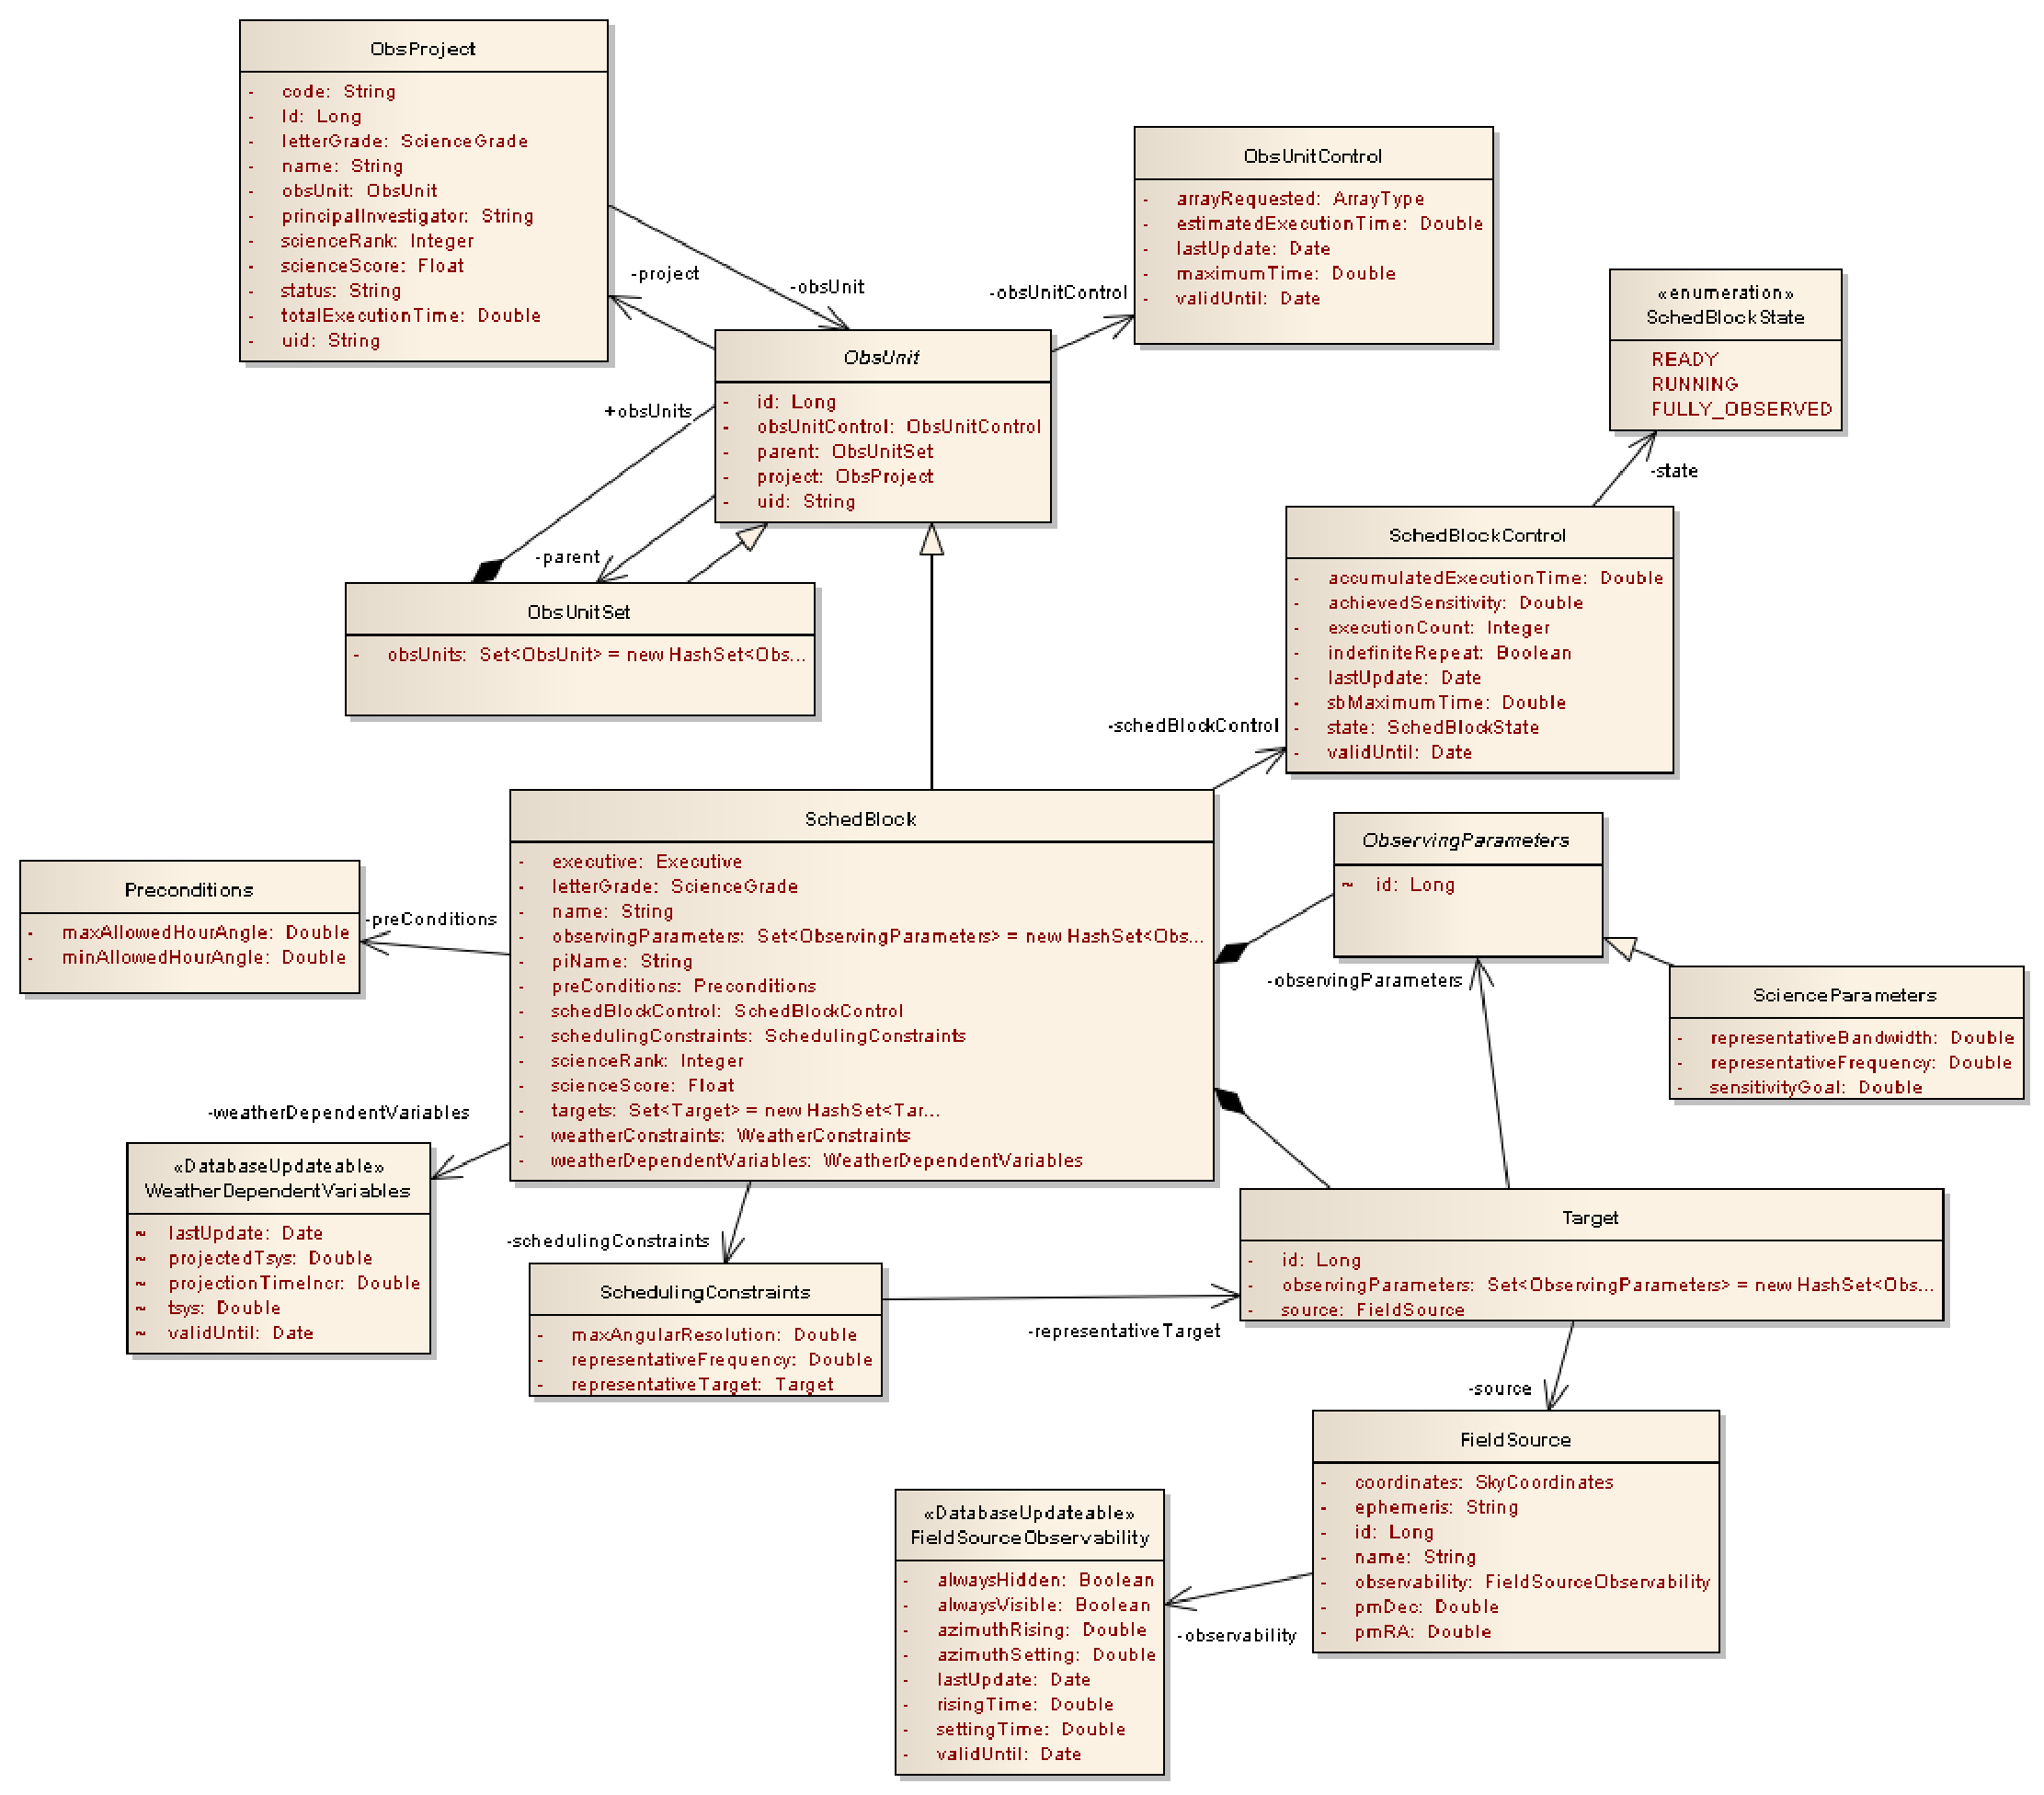
\includegraphics[width=1.15\textwidth]{images/ObsProject}
\caption{Observation Project data model}
\end{center}
\label{fig:datamodel-obsproject}
\end{figure}

The model designed for handle the observatory instrumentation is represented in figure~\ref{fig:datamodel-observatory}

\begin{figure}[]	
\begin{center}
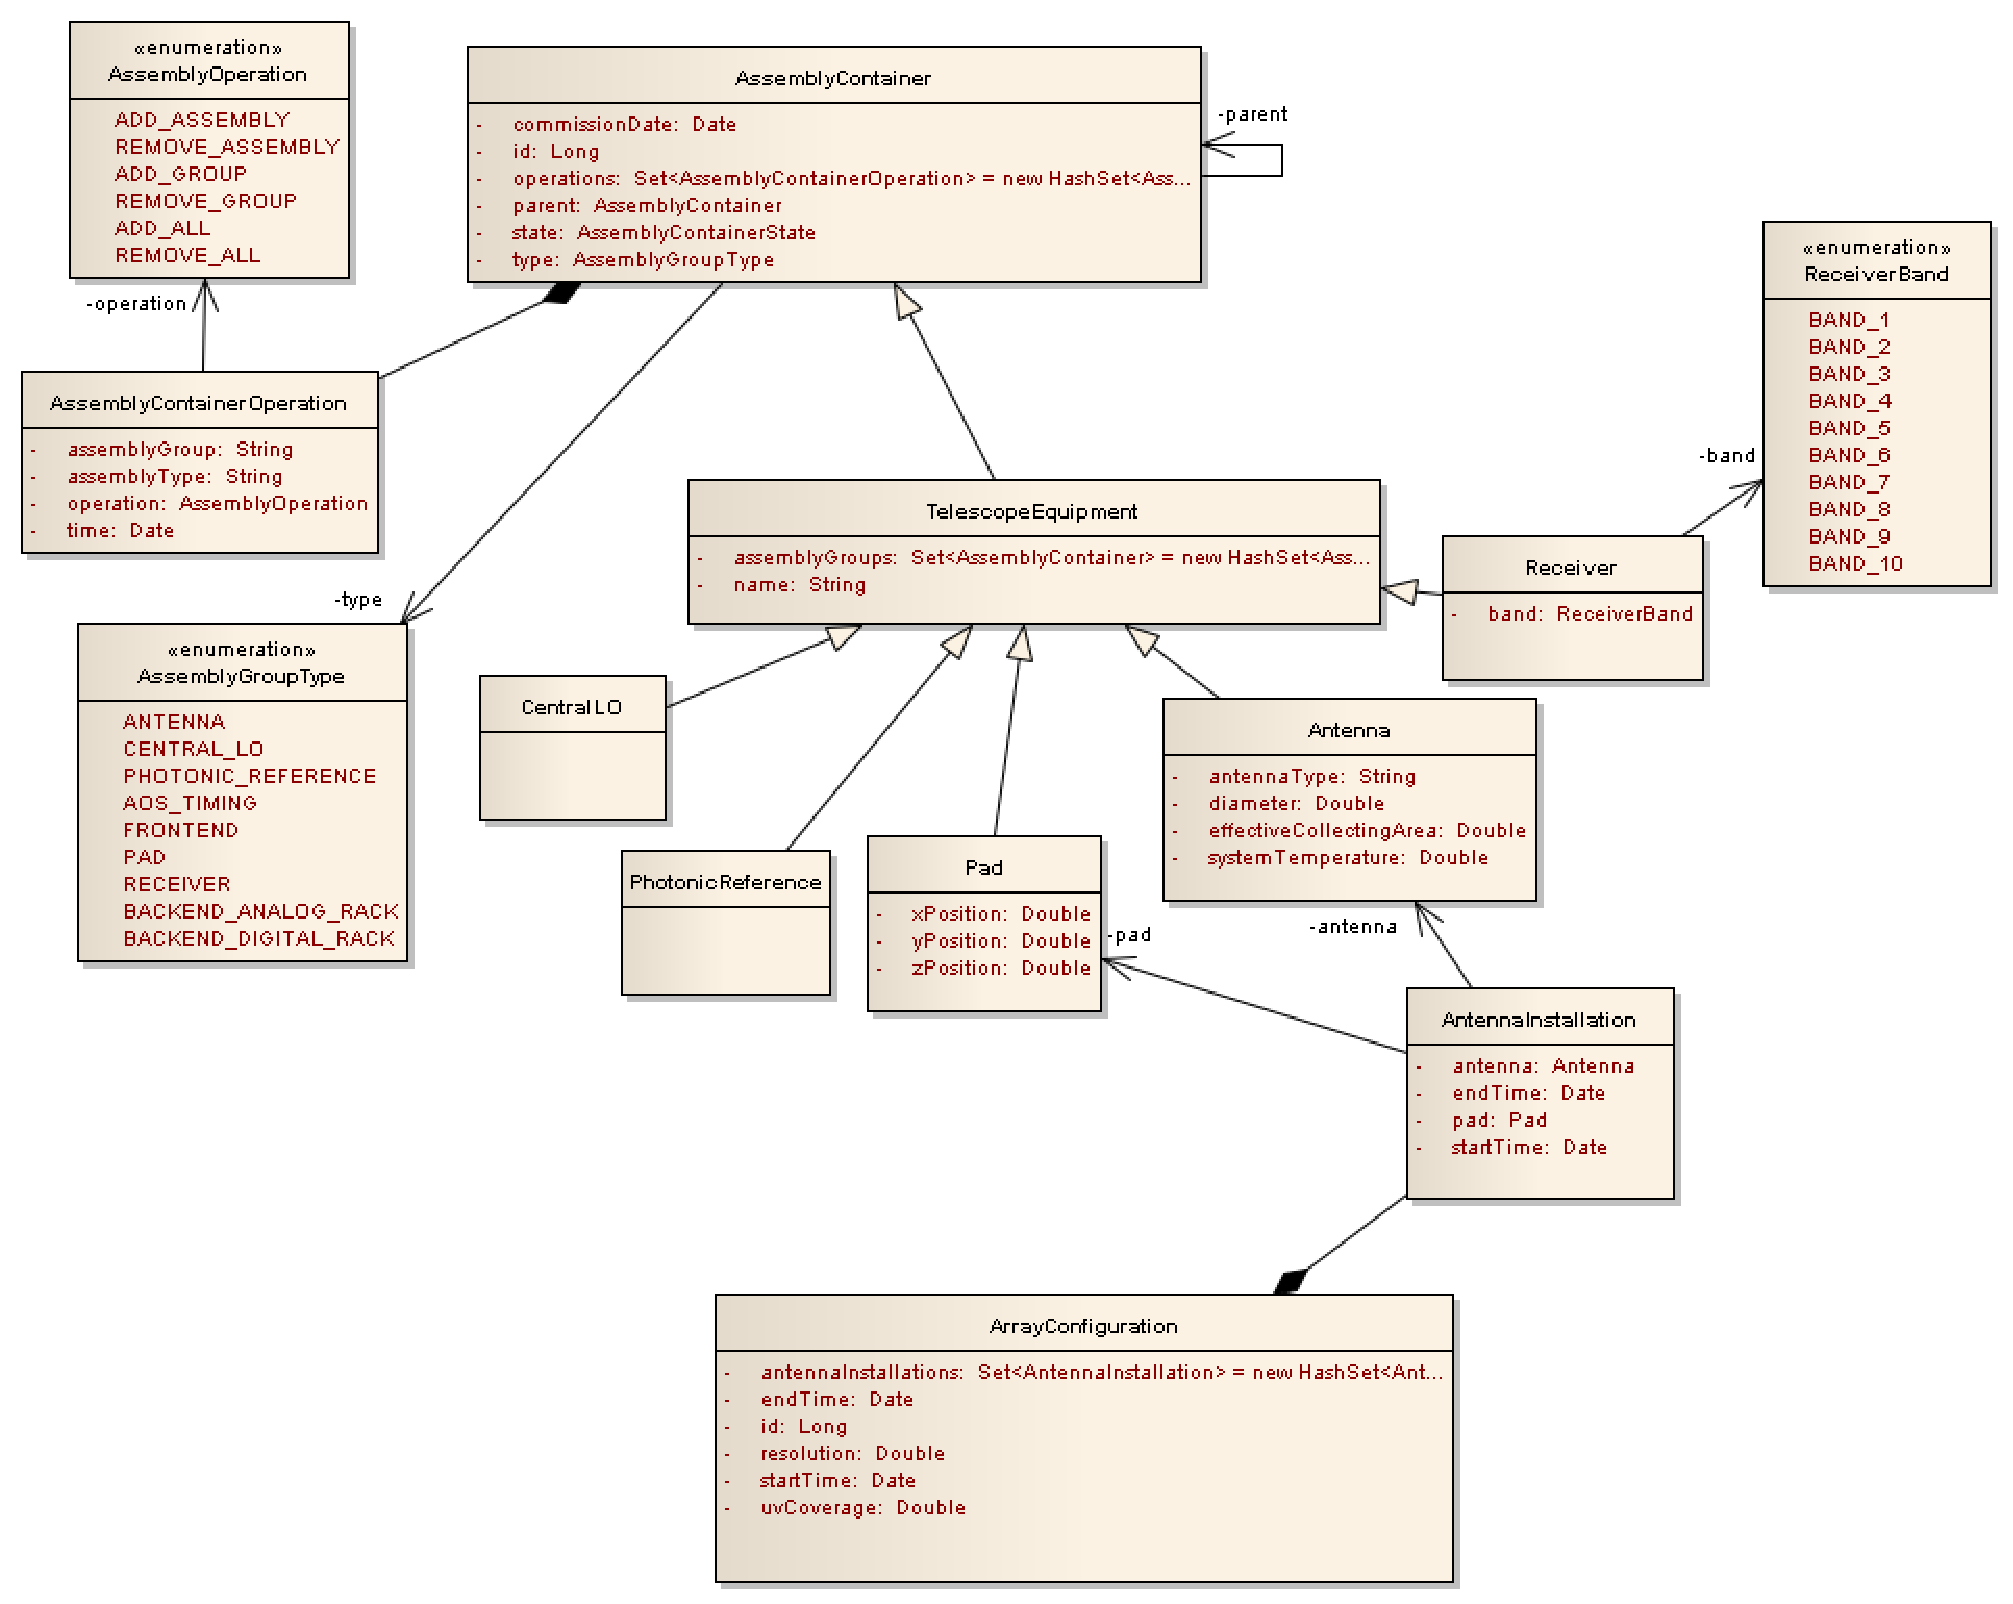
\includegraphics[width=\textwidth]{images/Observatory}
\caption{Observatory instrumentation data model}
\end{center}
\label{fig:datamodel-observatory}
\end{figure}

The model designed for handle the Executive information and the observing season is represented in figure~\ref{fig:datamodel-executive}

\begin{figure}[]	
\begin{center}
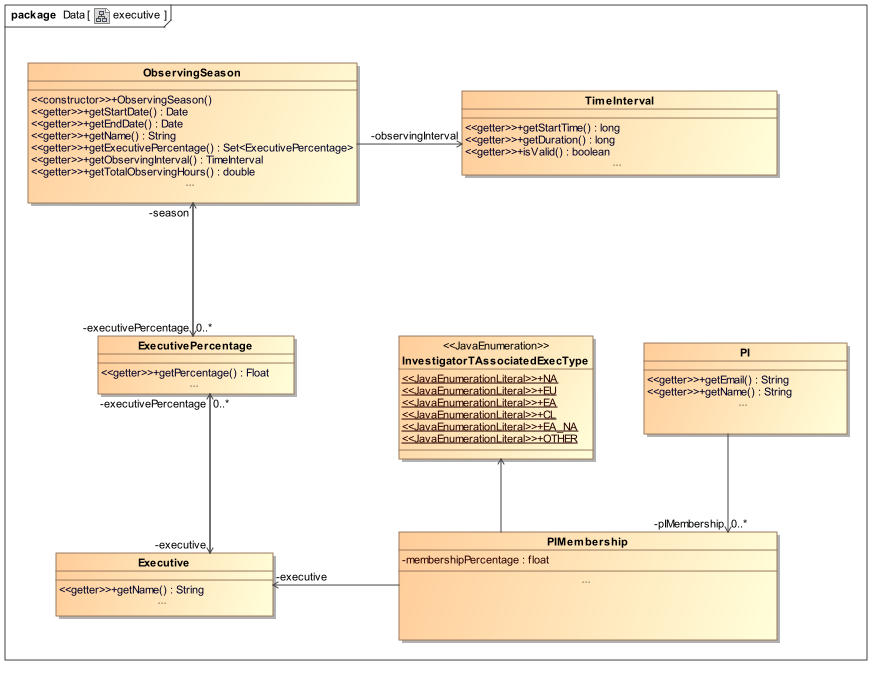
\includegraphics[width=\textwidth]{images/Executive}
\caption{Executive and observing season data model}
\end{center}
\label{fig:datamodel-executive}
\end{figure}

The model designed for handle the weather is represented in figure~\ref{fig:datamodel-weather}

\begin{figure}[]	
\begin{center}
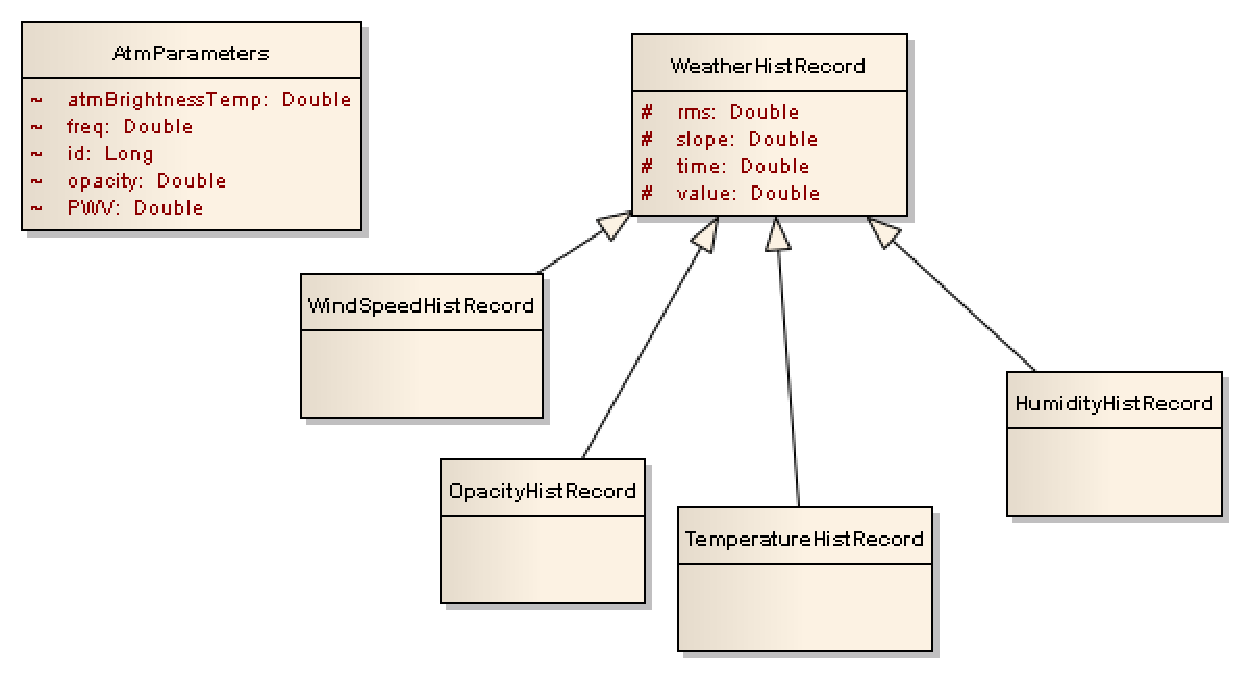
\includegraphics[width=\textwidth]{images/Weather}
\caption{Executive and observing season data model}
\end{center}
\label{fig:datamodel-weather}
\end{figure}

\section {Simulation}

\begin{figure}[]	
\begin{center}
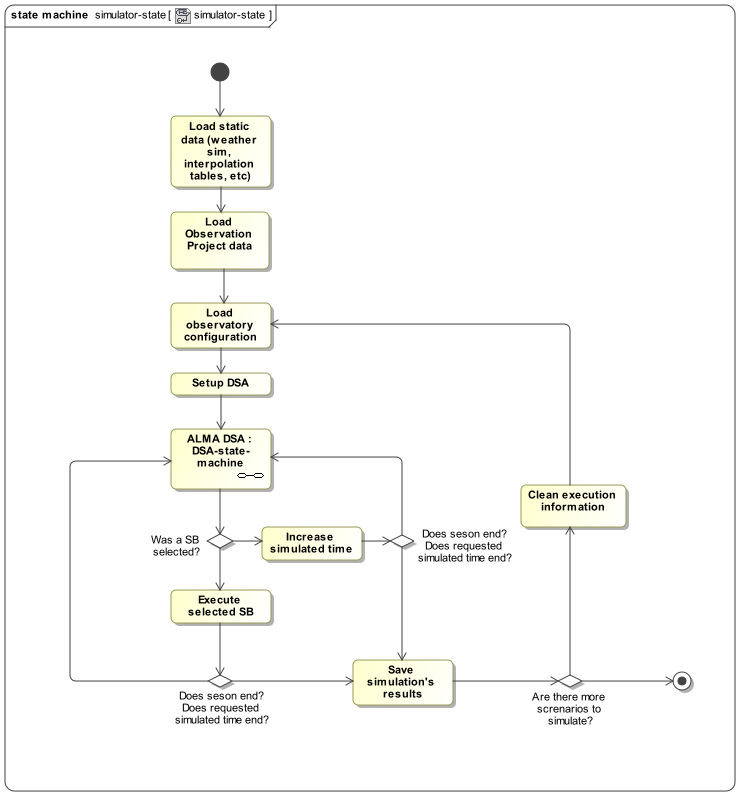
\includegraphics[width=\textwidth]{images/simulator-state-machine}
\caption{ALMA simulator's state machine}
\end{center}
\label{fig:sim-state-machine}
\end{figure}

\section {Algorithm implementation}

\section {Input Observation projects}

\begin{table}
\begin{center}
\begin{tabular}{|c|c|c|c|}
\hline
Configuration name & Array type & Min. Baseline $[m]$ & Max. Baseline $[m]$\\
\hline
C34-1 & $12\,[m]$ & $14.2$ & $165.6$ \\
\hline
C34-2 & $12\,[m]$ & $14.1$ & $303.6$ \\
\hline
C34-3 & $12\,[m]$ & $20.6$ & $442.7$ \\
\hline
C34-4 & $12\,[m]$ & $20.6$ & $558.2$ \\
\hline
C34-5 & $12\,[m]$ & $25.8$ & $820.2$ \\
\hline
C34-6 & $12\,[m]$ & $40.6$ & $1091.0$ \\
\hline
C34-7 & $12\,[m]$ & $40.6$ & $1507.9$ \\
\hline
7m    & $7\,[m]$  & $8.9$  & $32.1$ \\
\hline
TP    & $TP$      & $-$    & $-$ \\
\hline
\end{tabular}
\end{center}
\caption{Array configurations provided as input for the algorithms}
\label{table:input-array-configs}
\end{table}

\begin{table}
\begin{center}
\begin{tabular}{|c|c|c|c|}
\hline
Grade & Executive & Time Requested $[h]$ & Number of Scheduling Blocks \\ \hline
A &	CL		& 12.0  & 2 \\ \hline
A &	EA		& 36.0  & 13 \\ \hline
A &	EA/NA	& 6.0   & 3 \\ \hline
A & EU      & 112.0 & 31 \\ \hline 
A &	NA		& 114.0	& 31 \\ \hline
A & OTHER	& 0		& 0 \\ \hline
B  & CL 	& 160.0		& 48  \\ \hline
B  & EA     & 438.0     & 145 \\ \hline
B  & EA/NA  & 106.0     & 30  \\ \hline
B  & EU     & 828.0     & 280 \\ \hline
B  & NA     & 1024.0    & 344 \\ \hline
B  & OTHER  & 40.0      & 19  \\ \hline
C  & CL     & 130.0     & 50  \\ \hline
C  & EA     & 246.0     & 65  \\ \hline
C  & EA/NA  & 52.0      & 23  \\ \hline
C  & EU     & 410.0     & 155 \\ \hline
C  & NA     & 556.0     & 196 \\ \hline
C  & OTHER  & 34.0      & 13  \\ \hline
\end{tabular}
\end{center}
\caption{Requested time for $12m$ array configurations}
\label{table:requested-time-12m}
\end{table}

\begin{table}
\begin{center}
\begin{tabular}{|c|c|c|c|}
\hline
Grade & Executive & Time Requested $[h]$ & Number of Scheduling Blocks \\ \hline
A &	CL		& 0  & 0 \\ \hline
A &	EA		& 24.0  & 1 \\ \hline
A &	EA/NA	& 6.0   & 12 \\ \hline
A & EU      & 12.0 & 1 \\ \hline 
A &	NA		& 16.0 & 2 \\ \hline
A & OTHER	& 0		& 0 \\ \hline
B  & CL 	& 16.0		& 1  \\ \hline
B  & EA     & 78.0     & 21 \\ \hline
B  & EA/NA  & 22.0     & 5  \\ \hline
B  & EU     & 168.0     & 41 \\ \hline
B  & NA     & 182.0    & 29 \\ \hline
B  & OTHER  & 0.0      & 0  \\ \hline
C  & CL     & 38.0     & 2  \\ \hline
C  & EA     & 46.0     & 12  \\ \hline
C  & EA/NA  & 36.0      & 9  \\ \hline
C  & EU     & 5800     & 7 \\ \hline
C  & NA     & 556.0     & 196 \\ \hline
C  & OTHER  & 72.0      & 12  \\ \hline
\end{tabular}
\end{center}
\caption{Requested time for $7m$ array configurations}
\label{table:requested-time-7m}
\end{table}

\begin{table}
\begin{center}
\begin{tabular}{|c|c|c|c|}
\hline
Grade & Executive & Time Requested $[h]$ & Number of Scheduling Blocks \\ \hline
A &	CL		& 0  & 0 \\ \hline
A &	EA		& 28.0  & 1 \\ \hline
A &	EA/NA	& 208.0   & 2 \\ \hline
A & EU      & 132.0 & 1 \\ \hline 
A &	NA		& 112.0 & 2 \\ \hline
A & OTHER	& 0		& 0 \\ \hline
B  & CL 	& 28.0		& 1  \\ \hline
B  & EA     & 1852.0     & 21 \\ \hline
B  & EA/NA  & 752.0     & 5  \\ \hline
B  & EU     & 922.0     & 41 \\ \hline
B  & NA     & 1792.0    & 29 \\ \hline
B  & OTHER  & 0.0      & 0  \\ \hline
C  & CL     & 52.0     & 2  \\ \hline
C  & EA     & 1250.0     & 12  \\ \hline
C  & EA/NA  & 824.0      & 9  \\ \hline
C  & EU     & 368.0     & 7 \\ \hline
C  & NA     & 78.0     & 12 \\ \hline
C  & OTHER  & 2.0      & 1  \\ \hline
\end{tabular}
\end{center}
\caption{Requested time for $TP$ array configurations}
\label{table:requested-time-tp}
\end{table}

\begin{figure}
        \centering
        \begin{subfigure}[b]{0.45\textwidth}
                \includegraphics[width=\textwidth]{images/c34-1_sources}
                \caption{C34-1} 
        \end{subfigure} 
        ~ %
%
        \begin{subfigure}[b]{0.45\textwidth}
                \includegraphics[width=\textwidth]{images/c34-2_sources}
                \caption{C34-2}
        \end{subfigure}

        \begin{subfigure}[b]{0.45\textwidth}
                \includegraphics[width=\textwidth]{images/c34-3_sources}
                \caption{C34-3}
        \end{subfigure}
        ~ 
        \begin{subfigure}[b]{0.45\textwidth}
                \includegraphics[width=\textwidth]{images/c34-4_sources}
                \caption{C34-4}
        \end{subfigure}% 
        
        \begin{subfigure}[b]{0.45\textwidth}
                \includegraphics[width=\textwidth]{images/c34-5_sources}
                \caption{C34-5}
        \end{subfigure}
        ~
        \begin{subfigure}[b]{0.45\textwidth}
                \includegraphics[width=\textwidth]{images/c34-6_sources}
                \caption{C34-6}
        \end{subfigure}
        
        \begin{subfigure}[b]{0.45\textwidth}
                \includegraphics[width=\textwidth]{images/c34-7_sources}
                \caption{C34-7}
        \end{subfigure}           
        \caption{Visibility of A-graded Scheduling Blocks for $12\,[m]$ Array Configurations}
		\label{fig:results-sb-critical-set}
\end{figure}

\backmatter
\theglossary
%\begin{table}[h!t]
  \begin{tabular}{ll}
  ACA & Atacama Compact Array \\
  ALMA & Atacama Large Millimeter/submillimeter Array\\
  APDM & ALMA Project Data Model \\
  APEX & Atacama Pathfinder Experiment \\
  ATM & Atmospheric \\
  AURA & Association of Universities for Research in Astronomy \\
  CL & Chile \\
  CSP & Constraint Satisfaction Problem \\
  DAO & Data Access Object \\ 
  DRR & Deficit Round Robin \\
  DSA & Dynamic Scheduling Algorithm \\
  ESO & European Southern Observatory \\
  EA & East Asia \\
  EU & European Union \\
  GPS & Generalized Processor Sharing \\
  JRE & Java Runtime Environment \\
  LST & Local Sidereal Time \\
  NA & North America \\
  OCIW & Observatories of the Carnegie Institute of Washington\\ 
  PI & Principal Investigator \\
  PAE & Physical Address Extension \\
  PWV & Precipitable Water Vapor \\
  QPI & Intel's Quick Path Interconnect \\
  RH & Relative Humidity \\
  RMS & Root Mean Square \\
  SA & Simulated Annealing \\
  SAA & Simulated Annealing Algorithm \\
  SB & Scheduling Block \\
  SBs & Scheduling Blocks \\
  STScI & Space Telescope Science Institute \\
  TP & Total Power \\
  $T_{sys}$ & System Temperature \\ 
  VLA & Very Large Array \\
  XML & eXtensible Markup Language \\
  \end{tabular}
\end{table}

%\appendix
%\chapter{Astronomical calculations}

\section{Sensitivity}
\label{sec:sens-calc}
The RMS noise for multiple observations $\sigma$ is accumulated as shown in equation \ref{eq:rms-noise}.
\begin{equation}
\label{eq:rms-noise}
\sigma = \frac{\sqrt{\sum_{i=1}^M \sigma_i^2}}{M}
\end{equation}
where $M$ is the number of SBs and $\sigma_i$ is the RMS noise for a single
execution of an SB, calculated differently depending of the type of observation.
For interferometric observations the sensitivity is given by equation \ref{eq:sensitivity-interferometry}.
\begin{equation}
\label{eq:sensitivity-interferometry}
\sigma_i^{INT} = \frac{T_{sys}^i}{\eta_Q \sqrt{N_{INT}^i(N_{INT}^i-1)(\Delta\nu)\tau^i}}
\end{equation}
where $T_{sys}^i$ is the system temperature, $\eta_Q$ is the correlator sensitivity,
$N_{INT}^i$ is the number of antennas, $\Delta\nu$ is the bandwidth, and $\tau^i$ is
the integration time. All the quantities with the $i$ superscript are specific for the $i$-th
observation.

For single-dish observations
\begin{equation}
\sigma_i^{SD} = \frac{\alpha T_{sys}^i \sqrt{N_{SD}^i}}{\sqrt{(\Delta\nu)\tau^i}}
\end{equation}
where $\alpha$ is a numerical factor that depends on the scanning mode ($\sim 1$ for OTF,
$\sim \sqrt{2}$ for switched observations).

The RMS values are expressed in degrees Kelvin. To convert them to flux units, they are multiplied by the factor $2k/A_e$ where $k$ is the Boltzmann constant and $A_e$ is the antenna effective aperture.

These equations do not cover the case of the combined array, where the antennas in the array have different sizes, nor cover the cases where the bandwidth has been changed (multi-resolution modes, etc.).

\section{System Temperature}
\label{sec:tsys-calc}
The calculation of $Tsys$ is done in three steps:
\begin{enumerate}
\item First the Precipitable Water Vapor (PWV) content is determined. There are
several ways of doing this:
\begin{enumerate}
\item Calculate PWV from the Relative Humidity (RH) or the Dew Point. One way
of doing this is found in~\cite{butler98}. In this memo the PWV is developed as
$$
h = \frac{m_w P_0 H}{\rho_l k T_0}
$$
where $m_w$ is the mass of a water molecule (18 amu), $P_0$ is the water vapor
partial pressure, $H$ is the scale height of water vapor distribution (an
exponential distribution, 1.5 km for the VLA), $\rho_l$ is the density of
liquid water ($\mathrm{gr}/\mathrm{cm}^3$) and $k$ is the Boltzmann constant.

This memo presents a way to estimate $P_0$ from the dew point. In the subsequent
MMA Memo~\cite{butler98_1}, a way of calculating
$P_0$ from the relative humidity is given:
$$
P_0 = 2.409 \times 10^{12} \ RH\ \theta^4 \exp(-22.67\theta)
$$
where $\theta$ is the inverse temperature ($\theta = 300/T_0 $ K), and $RH$ is
the relative humidity.

\item Calculate it from the opacity $\tau_{225}$ at 225 GHz measured by the
tipper. In this case a way of calculating the $PWV$ can be seen in~\cite{delgado99}. $PWV$ can be obtained
by inverting
$$
\tau_{225} = 6.7787\cdot 10^{-3} + 4.0757\cdot 10^{-2} PWV + 9.59\cdot 10^{-4} PVW^2
$$
\item Get the PWV directly from the Water Vapor Radiometers.
\end{enumerate}
When the $PWV$ is available from different sources, the different values
are averaged.

\item Interpolate the ATM tables to determine the opacity $\tau$ and the
atmospheric effective temperature $T_{atm}$. The ATM tables have the following structure:
\begin{eqnarray*}
\tau & = & \tau(\nu_i, PWV_j) \\
T_{atm} & = & T_{atm}(\nu_i, PWV_j)
\end{eqnarray*}
where $\nu_i$ covers the range $20-1000$ GHz with 100 MHz granularity, and $PWV_j$
covers the 7 values 0.4772, 0.658, 0.9134, 1.262, 1.796, 2.748, and 5.186 (mm). 
\item The system temperature is calculated as:

$$
T_{sys} = \frac {\left ( T_{rx} + T_{ant} + \xi T_{ant} \right ) e^{\tau / \sin(el)}}
{\eta}
$$
where $T_{rx}$ is the receiver temperature, $\eta$ is the forward efficiency (or
feed efficiency, or spillover factor), $T_{ant}$ is the antenna temperature and $\xi$
is the sideband ratio, which for practical purposes will be $0$

Expanding the calculation of above:

$$
T_{sys} = \frac{\left ( T_{rx} + \eta T_{atm} \left ( 1 - e^{-\tau/\sin(el)} \right ) + (1 - \eta) 0.95 T_{amb} + \eta 2.76 e^{-\tau/\sin(el)} \right )  e^{\tau / \sin(el)}}
{\eta}
$$
where $T_{amb}$ is the ambient temperature, which is read from weather station.
\end{enumerate}

\section{Source visibility analysis}
\label{sec:sb-visibility}
From~\cite{meeus98} the altitude of a certain sky source is defined as shown by equation~\ref{eq:source-altitude}
\begin{equation}
\label{eq:source-altitude}
sin(h) = sin(\varphi) sin(\delta) + cos(\varphi) cos(\delta) cos(H)
\end{equation}
Where $h$ is the altitude, positive above the horizon, negative below; $\varphi$ is the observatory's latitude, positive is in northern hemisphere, negative in southern hemisphere; $\delta$ is the declination of the source, positive is north of the celestial equator, negative if south; and $H$ is the local hour angle, measured westwards from the South.

$H$ is calculated as shown by equation~\ref{eq:hour-angle-calculation}
\begin{equation}
\label{eq:hour-angle-calculation}
H = \theta - \alpha
\end{equation}
Where $\theta$ is the Local Sidereal Time (LST) and $\alpha$ is the right ascension of the sky source, usually it is expressed in terms of hours, minutes and seconds.

From these equations is possible to derive that the highest altitude in the sky is reach when $H = 0$. Or expressed in terms of LST, when $\theta = \alpha$. At this point is when there are less atmosphere between the observatory and the sky source, hence the quality of the data taken is better.

Nevertheless also it is possible to observe a sky source 
while it is not at its highest altitude in the sky, the key is to set a minimal altitude to allow to carry on observations properly. This minimum allowed altitude for ALMA observatory is set to $15^\circ$ mostly due to the surrounding mountains around the site. 

\section{Array Configuration duration and LST relationship}
\label{sec:array-visibility}
As stated in the general condition in section~\ref{sec:array-problem-general-condition} the minimum resolution for the problem is one (1) week.

From the algorithm used to calculate the LST found in~\cite{kaplan05}, it is possible to deduce that the LST drifts from the calendar time. The drift calculated rate is approximately $1654.7328\,[s]$ or $27.57888\,[min]$ ahead for every calendar week.

Therefore, the LST interval during the minimum array lifespan (of 4 weeks) will be approximately the number of hours in the daily time interval plus $1.838592\;[h]$.
Of course the borders of the configuration interval, in LST terms, would not be available the whole array duration due to the LST drifting, and these LST hours will have less representation as the array configuration life advances. But for a crude estimation of the LST interval available during array configuration life, works fine.

The minimum configuration duration set by the problem and its model definition (4 weeks), may be changed according to the total time requested by the Scheduling Blocks covered under the calculated LST range for the given array configuration. Then, the array configuration lifespan could be either the minimum duration defined by the problem, or the total time requested by the Scheduling Blocks, or a value between both.

\chapter{ALMA Project Data Model brief description}
\label{sec:apdm}
The ALMA Software system works using the concept of an Observing Project, the full description and the details of the model are available at~\cite{bridger09}. The Observing Project is used throughout the ALMA software as the top level structure associated with a project resulting from a single observing proposal. In fact the Observing Project is a container for all the information relating to a project before it begins execution. During and following execution other data associated with the project are created and held in other structures, each of which holds a reference to the original observing project. Of particular interest is the Project Status structure, which holds a record of the execution status of the Project. The ALMA Project Data Model (APDM) defines the structure of both the Observing Project (ObsProject) and the execution status (ProjectStatus).

The Scheduling Block (SchedBlock or SB) is the atomic unit of observing for ALMA, any given science observation will usually be broken into many SBs, which may, or may not be executed in sequence. The ALMA Scheduling Software will decide on which SB to execute at any given time on the basis of which is the best to execute now.

\begin{description}
\item[Observation Project Entity] \hfill \\
When a ALMA user submits a project to the Data Base, then the user is creating a ObsProject. Almost all the end-user tools in ALMA operates on ObsProjects, no other entities are exposed to the end user.

In order to hold all of the pre-observing information associated with a project the ObsProject entity class is composed of three parts: an ObsProposal, an ObsReview and an ObsProgram. These hold the information associated with the three phases of observing preparation: the proposal or Phase I; the reviewing and resultant approvals where the \textit{scientific value} is assigned by the \textit{Time Assignment Committee}; and the observing program definition, or Phase II.

\item[Observation Program Entity] \hfill \\
The Observing Program (ObsProgram) part of the Observing Project holds all the information created during Phase II, or program preparation. The ObsProgram consists of an Observing Plan (ObsPlan) and a SciencePlan. The Science Plan covers the science goal oriented view of the observing, and it is intended to contain the information that most users will use to define their observing programs. This information will persist, for the convenience of users, but will not be the definition that is used by the Observatory when carrying out the observations. Instead the latter information is contained within the ObsPlan, and covers what we call the system view. The service of Program Generation allows users to create the Observing Plan from their Science Plan. It is also possible for very advanced users to ignore the Science Plan and simply create all of the Observing Plan directly.

As stated, the Observing Plan (ObsPlan) is the container for defining the actual observing objects. In modeling terms the ObsPlan is a role for the top level ObsUnitSet, heading the definition of the system view. An ObsUnitSet contains a collection of Scheduling Blocks or more ObsUnitSets, along with objects defining the preconditions, performance and calibration requirements, and flow control that apply to that collection.


\item[Scheduling Block Entity] \hfill \\
A Scheduling Block (SB) is the unit of observing for ALMA. It defines all the information that is required by the Observatory to independently execute the acquisition of a set of data and then to calibrate it as well. Since SBs are selected for execution individually they must exist as separate items in the data base.

Most of the structures within the SB hold information that is used either by the scheduler, to query whether or not this SB is suitable for scheduling ``now'', or as information that is used by the Observing Script (in the Control subsystem) to actually execute the observing (see below), and in some cases both. There are also performance goals for the SBs, to be measured against by the observing system.

So to allow the determination of ``Schedulability'' we find items like representative target observability, weather constraints, a precondition that requires a current Baseline Calibration and a Scientific Priority.

\item[Targets] \hfill \\
The target is the element within an SB that defines the area to map, the spectral or instrumental setups to use, and the purpose of the observing. In fact the target element itself contains nothing except references to other elements that contain descriptions of these three key components.

\end{description}

\chapter{ALMA Scheduling software work-flows}
\section{DSA workflow}
\label{sec:dsa-workflow}

\begin{figure}[htbp]	
\begin{center}
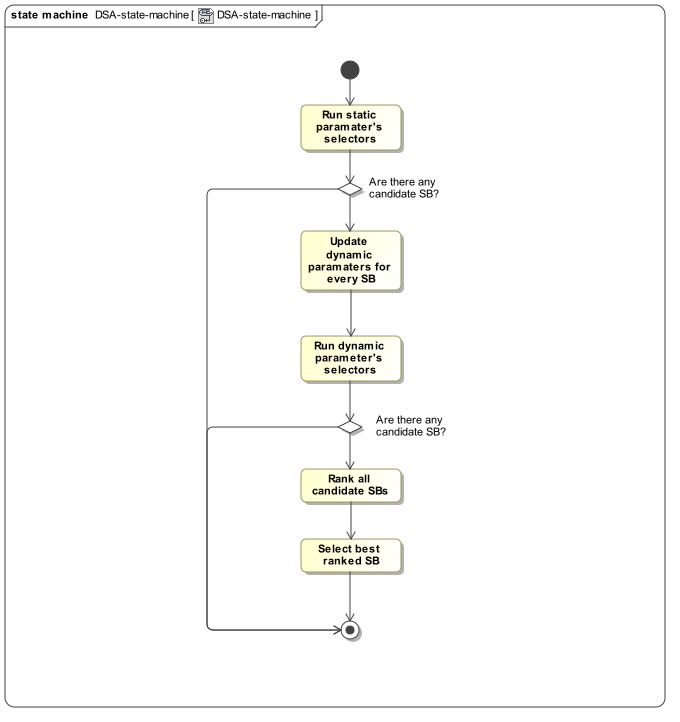
\includegraphics[width=0.9\textwidth]{images/DSA-state-machine}
\end{center}
\caption{Dynamic scheduling algorithm's state machine}
\label{fig:sched-dsa-state-machine}
\end{figure}

\begin{description}
\item[Run static parameter's selector] \hfill \\
After running these selectors the algorithm will return a list of the potential candidates given current static conditions, this includes the visibility for the representative target which is known beforehand, but is not filterable until the algorithm knows the current Local Sidereal Time. If after this state there is no feasible solution, then the algorithm will return nothing.

\item[Update dynamic parameters] \hfill \\
In this state the algorithm will recalculate the parameters requiring update at the given time. Usually weather conditions and parameters that cannot be calculated beforehand (e.g. altitude of a source for the given time, the point in the sky is in RA-Dec coordinates).  

\item[Run dynamic parameter's selector] \hfill \\
This will filter out all the Scheduling Blocks which do not fit in the criteria established after the dynamic updates ran. As the first state it will return a list of the candidate SB. If after this state there is no feasible solution, then the algorithm will return nothing.

\item[Rank all candidate Scheduling Blocks] \hfill \\
The algorithm might have a list of scorers, each one of these ``scorers'' will assign a value between ${[ 0 , 1 ]}$. The algorithm also will have a list of weights, one per scorer. The final result of each Scheduling Blocks will be sum of all the weighted scores given to this Scheduling Block for the given time to the algorithm.

\item[Select best ranked Scheduling Block] \hfill \\
The algorithm will select, and will return, the ``best'' suitable Scheduling Blocks for the given time.

\end{description}

\section{Simulator workflow}
\label{sec:sim-workflow}
The simulator is the one used in the ALMA's scheduling subsystem. At the time when this document was written it remains mostly unchanged from its original design explained in detail in~\cite{hoffstadt10}. Nevertheless some modifications were done during the development of this work, to support the simulation of several scenarios for the solution provided for the ``Array configuration planning problem''. Next a briefly description of the simulator work-flow, shown in figure~\ref{fig:sim-state-machine}, is presented:

\begin{figure}[h!]	
\begin{center}
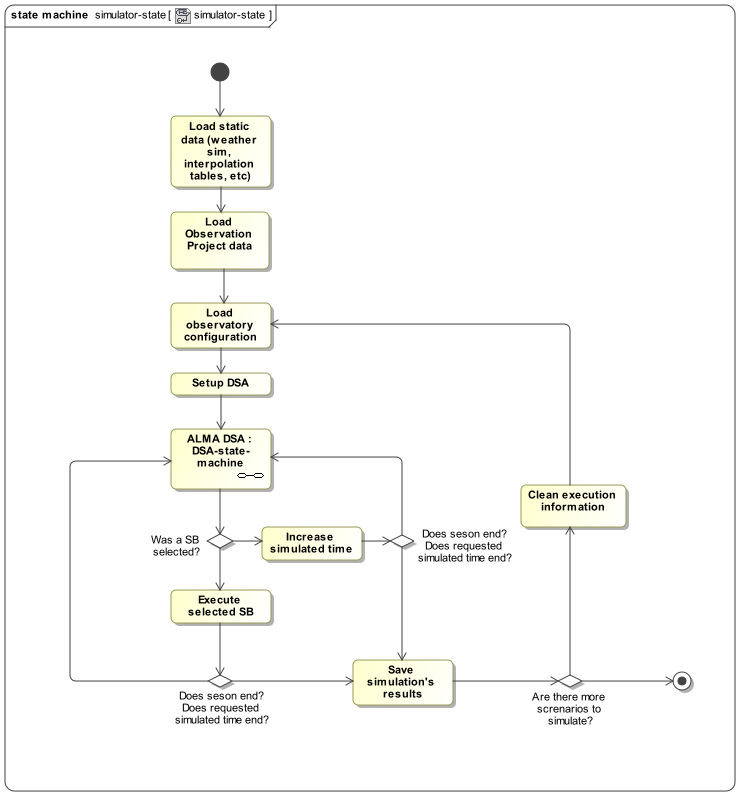
\includegraphics[width=0.67\textwidth]{images/simulator-state-machine}
\end{center}
\caption{ALMA simulator's state machine}
\label{fig:sim-state-machine}
\end{figure}

\begin{description}
\item[Load static data] \hfill \\
In this step the simulator will load all the immutable data from data-sources. This includes weather simulation data (temperature, humidity, wind speed, etc) and atmospheric interpolation tables to calculate the atmospheric opacity given the PWV and frequency. This step is separate from the rest of the data given that, the original ALMA's simulator is intended to be run using a relational database as back-end, then the data will be loaded just once.

During the development of this work, the simulator has been modified to work with data loaded completely in memory. Therefore this step add no value to the simulator itself. However it is worth of mention the difference with the original simulator used in ALMA software. 

\item[Load Observation project data] \hfill \\
In this step the simulator will load the data intended to be modified within the simulation procedure. This includes the whole observation projects, information relative to the executives and observing season.

\item[Load observatory configuration] \hfill \\
In this step the simulator loads or modifies the array configuration planning for the observing season. Originally, the ALMA's simulator supported only the loading of this data from the data-sources. During the development of this work this step was separated from the previous one, to support the setup of multiple scenarios for the, already configured, observing season.

\item[Setup DSA (algorithm for Astronomical observation scheduling problem)] \hfill \\
In this step the different simulations for each array configuration are scheduled. The simulator, according to its progress, will change among the different array configurations prepared in this step. If the simulator detects that there are no more configurations remaining for the rest of the simulated duration, then it will terminate the simulation execution and it will prepare the results and output them.

\item[Running DSA (DSA-state-machine)] \hfill \\
In this step the DSA will execute according to the work-flow presented in figure~\ref{fig:sched-dsa-state-machine} and explained in section~\ref{sec:astro-schedule-problem}.

If the DSA returns no result, then the simulator will jump $1\,[h]$ and $20\,[m]$ its simulation and try again checking whether there are selectable scheduling blocks or not. The simulator will do this until the array end time is reached.

\item[Save simulation's result] \hfill \\
After every simulation is complete, the simulator will dump a XML file containing most of the information for post-analysis.

\item[Clean execution information] \hfill \\
Since during simulation certain data for the Scheduling blocks are filled (like current number of repetitions and total time duration) and executive accounting is modified. It is necessary to clean-up all the modified data. 

The implementation done for this work will clean the complete context used for simulation, and it will reload all the data from scratch. Although it is known that this produce an overhead for the testing, it is safer to reload all the data to avoid to find programming defects during testing.
\end{description}

\chapter {Data model and implementation details}
\label{sec:implementation}
The model designed for the observation project hierarchy, is represented in figure~\ref{fig:datamodel-obsproject}, this is a simplification of the ALMA Project Data Model summarized in appendix~\ref{sec:apdm} and it is the model used in the ALMA's Dynamic Scheduling Algorithm, briefly described in section~\ref{sec:alma-dsa}.

The most relevant parts are: 
\begin{description}
\item[ObsProject] \hfill \\
This is top-level container for a group of observations requested. This container defines the scientific grade and rank, as well particular information of the executive, whom has requested the observation. All this information is shared with the set of scheduling blocks contained within.
\item[SchedBlock] \hfill \\
This is the atomic scheduling unit for the scheduling algorithm. The SB will contain information related to scheduling constraints, like array type requested, representative band, max/min angular resolution, etc; weather constraints, like, max. opacity, max. wind speed, etc; time constraints, like max. observation time, temporal boundaries; and the sky source.
\end{description}

\begin{figure}[htbp]	
\begin{center}
\includegraphics[width=1.15\textwidth]{images/Obsproject}
\end{center}
\caption{Observation Project data model}
\label{fig:datamodel-obsproject}
\end{figure}

The model designed to handle the observatory instrumentation is represented in figure~\ref{fig:datamodel-observatory}. This is an over simplification of what is presented in~\cite{avarias11, hoffstadt10}, the \textbf{ArrayConfiguration} class covers the minimal needs to allow to the algorithm to take a decision regarding the array configuration parameters. The simplification was done because the original classes defined did not add any extra value for the algorithm.

\begin{figure}[htbp]	
\begin{center}
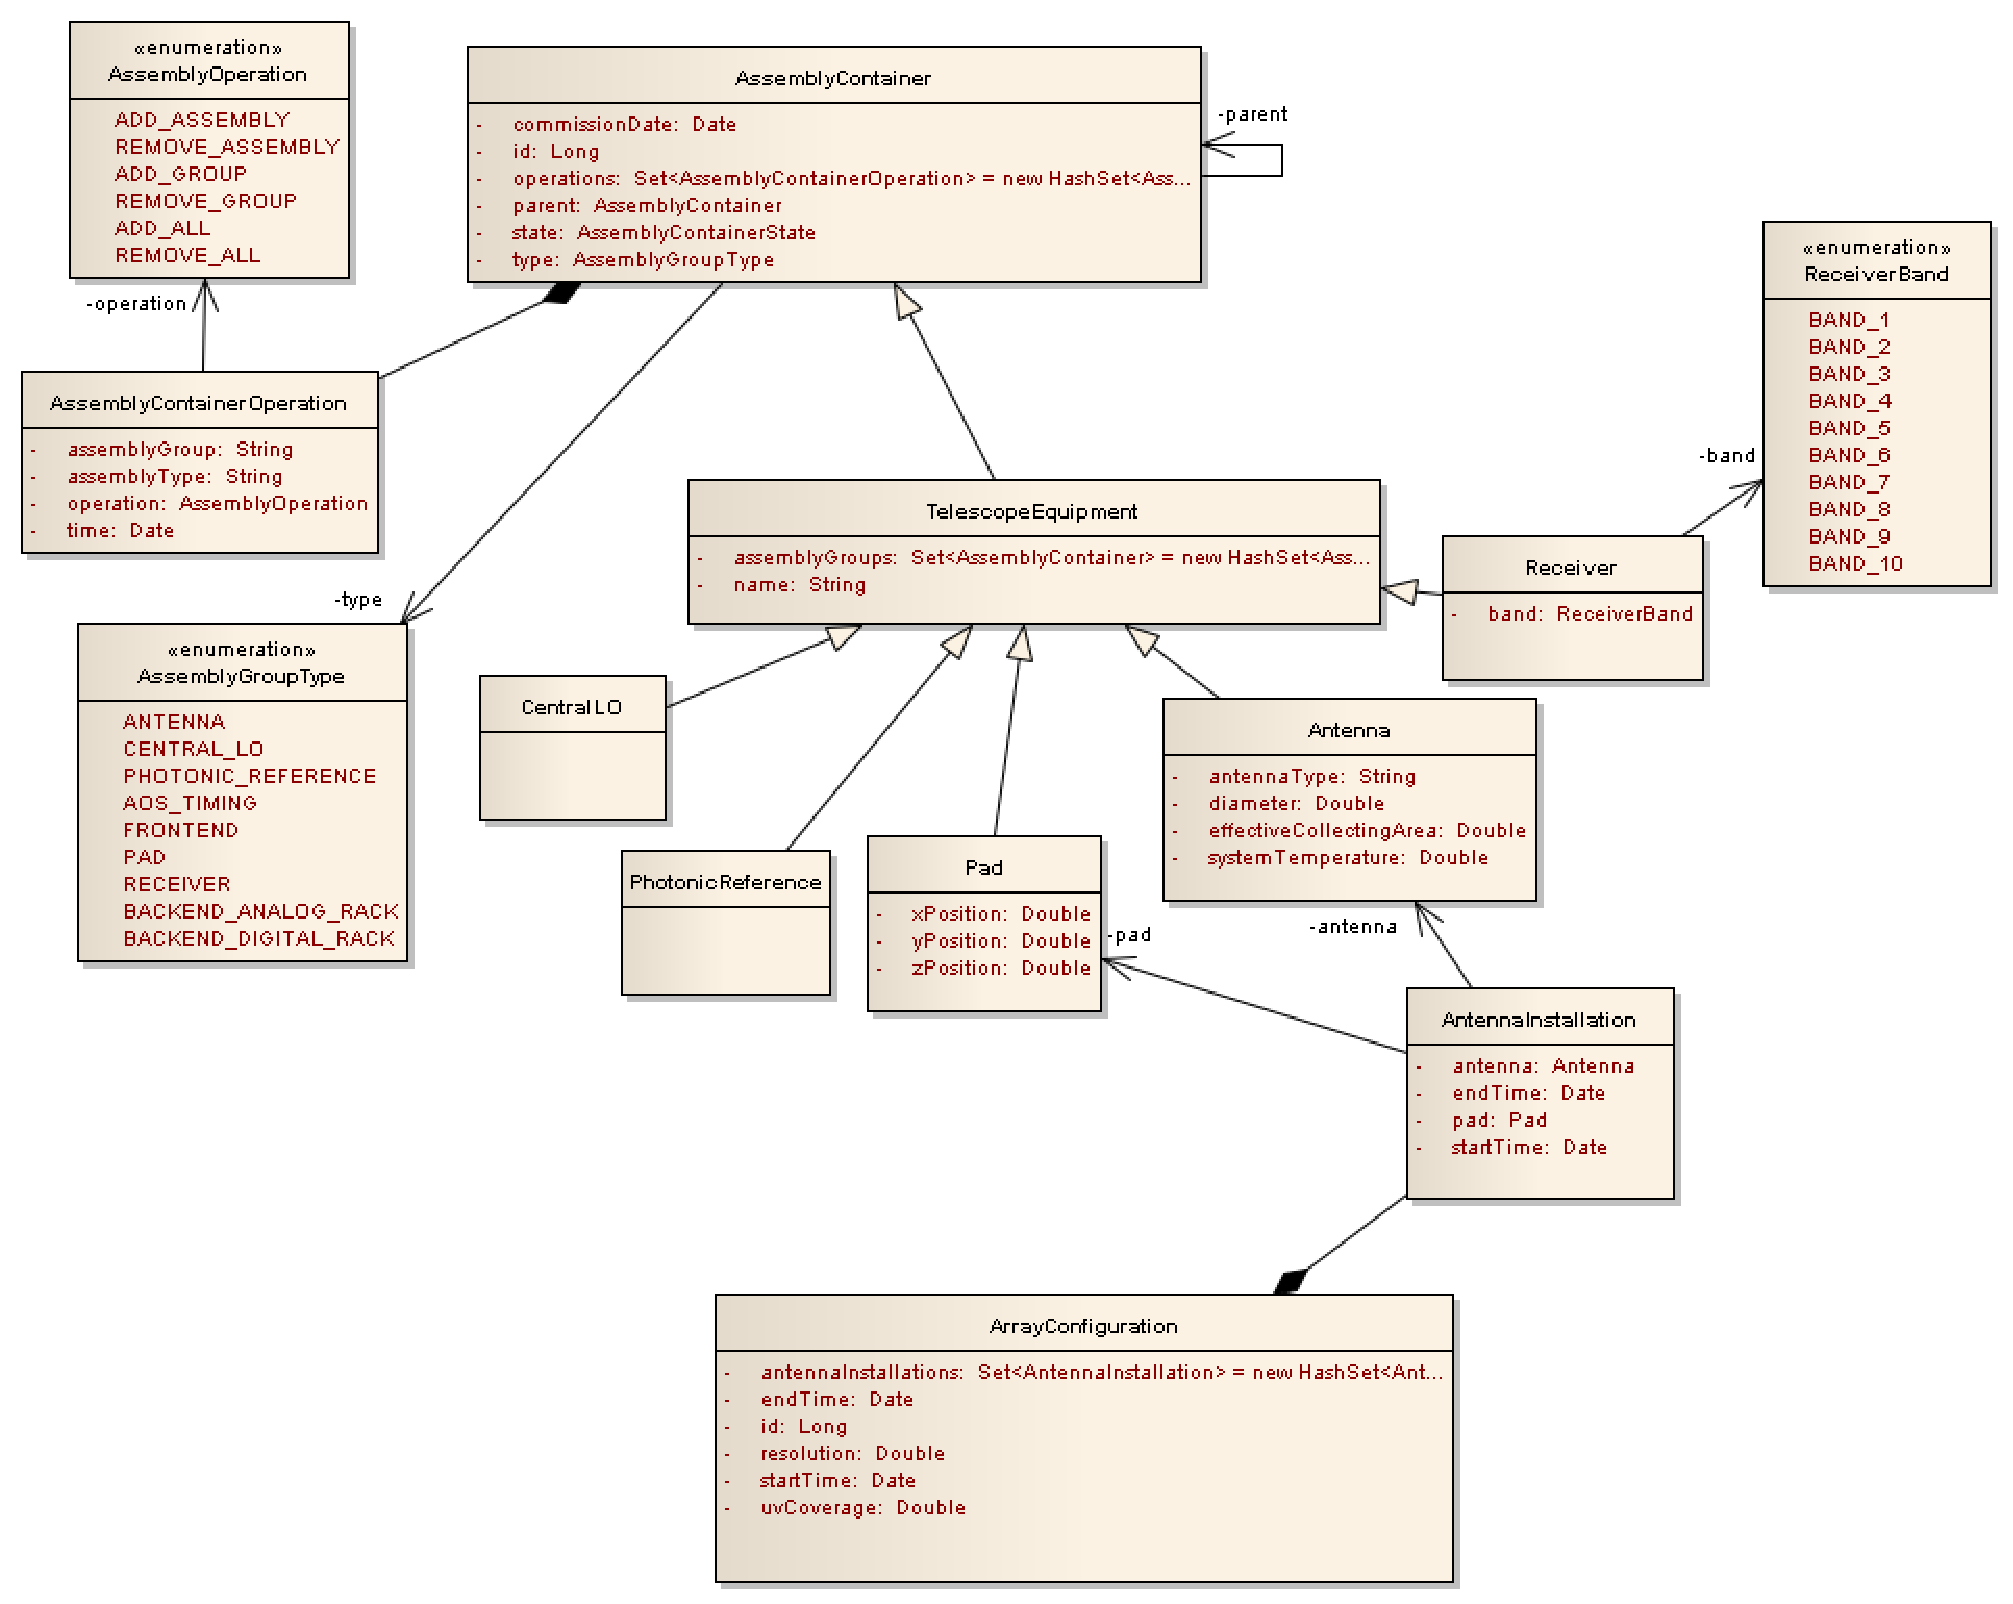
\includegraphics[width=0.67\textwidth]{images/Observatory}
\end{center}
\caption{Observatory instrumentation data model}
\label{fig:datamodel-observatory}
\end{figure}

The model designed for handle the Executive information and the observing season is represented in figure~\ref{fig:datamodel-executive}
The most relevant parts are: 
\begin{description}
\item[Executive] This class holds the information related to each executive provided as input. It saves the percentage and associates each Principal Investigator (class \textbf{PI}). Originally, the model was designed to allow to every PI have assigned percentages to each executive. However in practice, this has not been used.

\item[Observing Season] This class has the information related to the start and end dates for the observing season or observing cycle, also keeps the information relative to the daily schedule, in a \textbf{TimeInterval} class instance.
\end{description}

\begin{figure}[htbp]	
\begin{center}
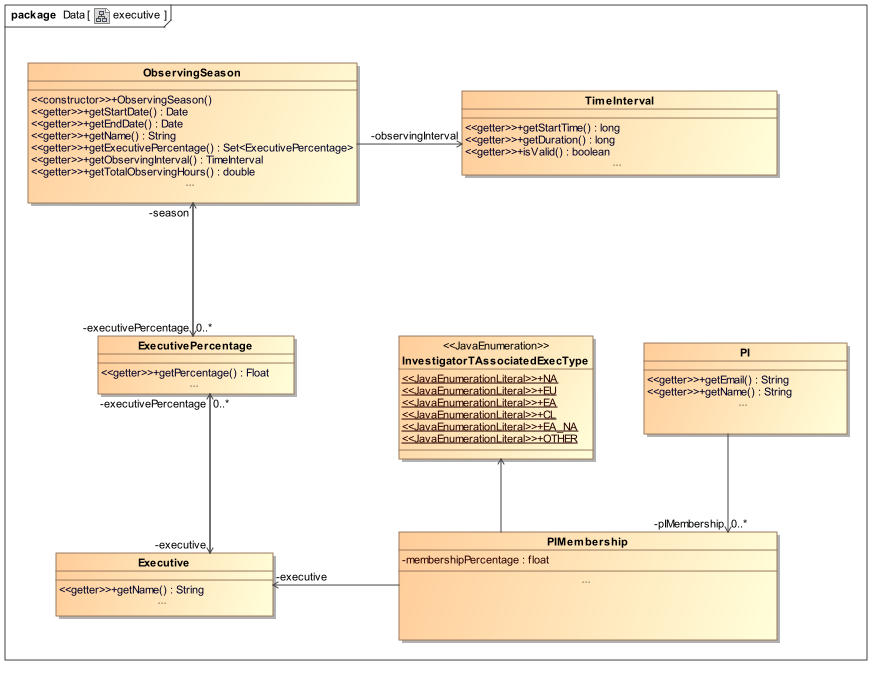
\includegraphics[width=0.67\textwidth]{images/Executive}
\end{center}
\caption{Executive and observing season data model}
\label{fig:datamodel-executive}
\end{figure}

The model designed to handle the weather is represented in figure~\ref{fig:datamodel-weather}. The weather model is quite simple, it has several classes holding data for the simulated weather, like precipitable water vapor, temperature, wind speed and phase. Also the model has the class \textbf{AtmParamters}, which contains the interpolation tables to calculate the atmospheric opacity.

\begin{figure}[htbp]	
\begin{center}
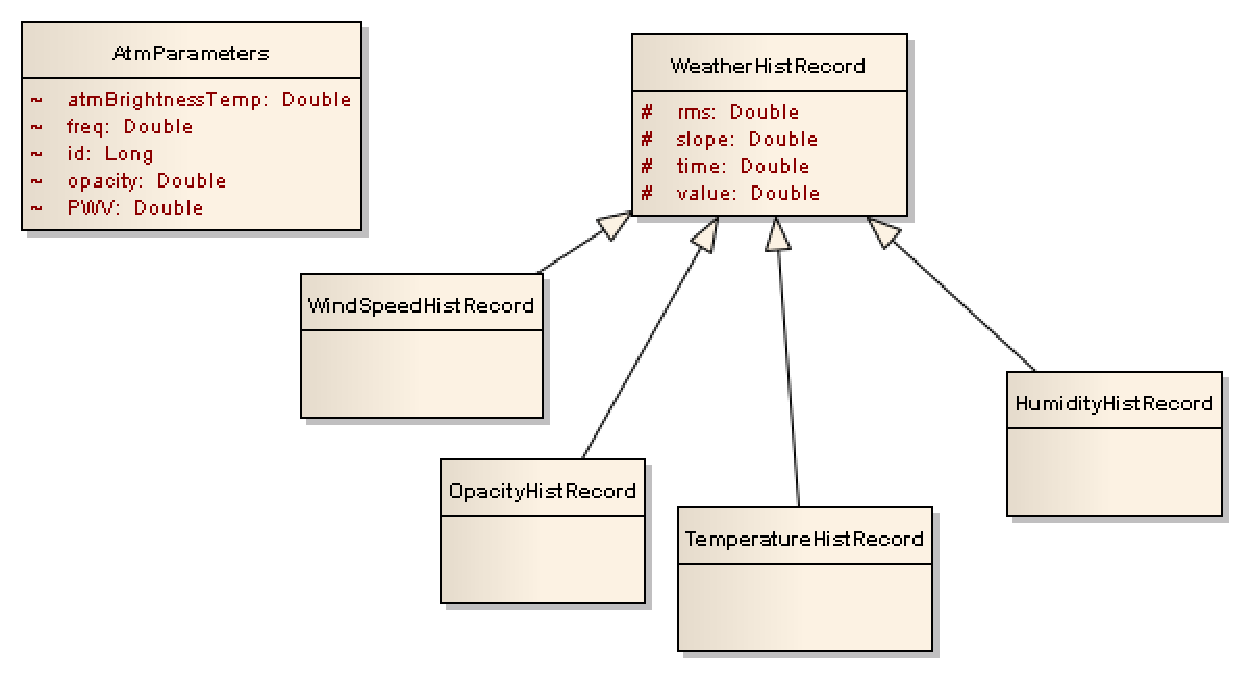
\includegraphics[width=0.67\textwidth]{images/Weather}
\end{center}
\caption{Weather data model}
\label{fig:datamodel-weather}
\end{figure}

The model designed to handle the observation progress status is represented in figure~\ref{fig:datamodel-observation}. This model defines the \textbf{ExecBlock}, which keeps the time accounting and progress for each SB, array configuration and Executive. 

\begin{figure}[htbp]	
\begin{center}
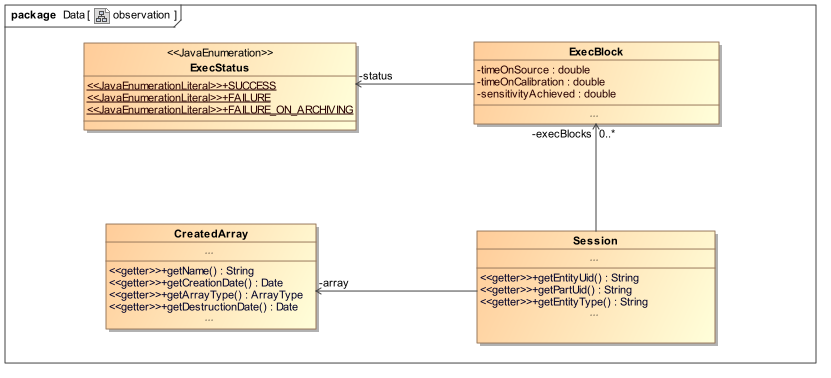
\includegraphics[width=0.67\textwidth]{images/Observation}
\end{center}
\caption{Observation progress status}
\label{fig:datamodel-observation}
\end{figure}

The top-level architecture of the ALMA's scheduling planning simulator is represented in diagram~\ref{fig:sim-top-level-architecture}. The software design uses as glue the Spring Core library, using Inversion of Control paradigm is possible to define via a configuration file, the objects to inject into the simulator, this includes Data Access Objects instances and the algorithm instances. It is enough for the software developed in this work to implement the correct interfaces to make them compatible with the rest of the ALMA software.

For the development of the validation software prepared for this work, some changes were done. Essentially the whole DAO's code, presented in the left part and on bottom part of the figure~\ref{fig:sim-top-level-architecture}, which is particular to ALMA software, were replaced with a Data Accessors able to read the XML format defined by the scheduling subsystem software, for data-interchange; and with in-memory data structures provided by the Java API, respectively. The core of the simulator tool and the algorithm does not deal directly with the data, instead a Data Accessors Object (DAO) interface was defined already by the ALMA's scheduling software, which abstracts all the interaction between the simulator and the data. Hence the replacement was fairly easy.

\begin{figure}[h!]	
\begin{center}
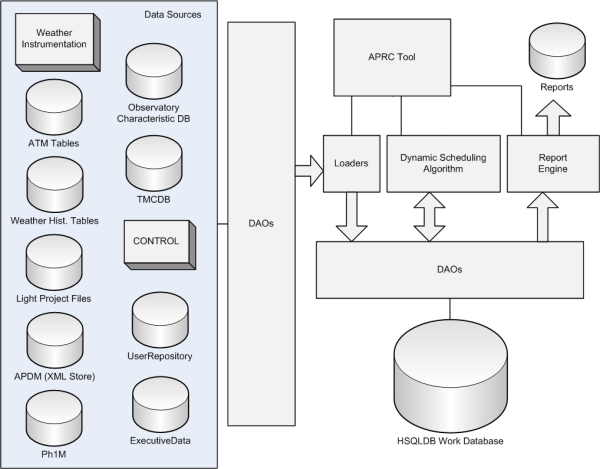
\includegraphics[width=0.67\textwidth]{images/simulator-arch}
\end{center}
\caption{Current top-level ALMA's scheduling simulator tool}
\label{fig:sim-top-level-architecture}
\end{figure}

In other hand, the algorithm implemented by ALMA software (DSA) was replaced with the modified Deficit Round-Robin algorithm implementation presented in this work (see chapter~\ref{sec:astro-schedule-problem}). The ALMA software design also make provisions at the algorithm level, defining an interface, which, as well as the DAOs, was fairly easy to replace with new classes developed to implement the modified DRR algorithm.

\chapter{Scheduling Block critical subset for each array configuration}
\label{sec:sb-critical-set}
\begin{figure}[htbp]
        \centering
        \begin{subfigure}[b]{0.45\textwidth}
                \includegraphics[width=\textwidth]{images/c34-1_sources}
                \caption{C34-1} 
        \end{subfigure} 
        ~ %
%
        \begin{subfigure}[b]{0.45\textwidth}
                \includegraphics[width=\textwidth]{images/c34-2_sources}
                \caption{C34-2}
        \end{subfigure}

        \begin{subfigure}[b]{0.45\textwidth}
                \includegraphics[width=\textwidth]{images/c34-3_sources}
                \caption{C34-3}
        \end{subfigure}
        ~ 
        \begin{subfigure}[b]{0.45\textwidth}
                \includegraphics[width=\textwidth]{images/c34-4_sources}
                \caption{C34-4}
        \end{subfigure}% 
        
        \begin{subfigure}[b]{0.45\textwidth}
                \includegraphics[width=\textwidth]{images/c34-5_sources}
                \caption{C34-5}
        \end{subfigure}
        ~
        \begin{subfigure}[b]{0.45\textwidth}
                \includegraphics[width=\textwidth]{images/c34-6_sources}
                \caption{C34-6}
        \end{subfigure}
        
        \begin{subfigure}[b]{0.45\textwidth}
                \includegraphics[width=\textwidth]{images/c34-7_sources}
                \caption{C34-7}
        \end{subfigure}           
        \caption{Visibility of A-graded Scheduling Blocks for $12\,[m]$ Array Configurations}
		\label{fig:results-sb-critical-set}
\end{figure}

The LST intervals proposed by the Scheduling Block classification software can be seen in table~\ref{table:lst-int-prop}.

\begin{table}[htbp]
\begin{center}
\begin{tabular}{|c|c|c|}
\hline
\textbf{Array configuration} & \textbf{Start time (LST)} & \textbf{End time (LST)} \\ \hline
C34-1 & 5.61692 & 15.45551 \\ \hline
C34-1 & 13.30675 & 23.14534 \\ \hline
C34-2 & 9.86519 & 19.703777 \\ \hline
C34-2 & 13.22811 & 23.06670 \\ \hline
C34-3 & 4.44851 & 14.28710 \\ \hline
C34-3 & 9.76941 & 19.60800 \\ \hline
C34-3 & 12.97411 & 22.81270 \\ \hline
C34-4 & 5.61692 & 15.45551 \\ \hline
C34-5 & 9.93925 & 19.77784 \\ \hline
C34-6 & 21.92851 & 7.76710 \\ \hline
C34-7 & 2.77808 & 12.61667 \\ \hline
C34-7 & 4.94547 & 14.78406 \\ \hline
C34-7 & 9.76941 & 19.60800 \\ \hline
\end{tabular}
\end{center}
\caption[LST intervals proposed by the Scheduling Blocks categorization]
{LST intervals proposed by the Scheduling blocks categorization described in section~\ref{sec:array-sb-classification}}
\label{table:lst-int-prop}
\end{table}

Comparing both, the sources elevation vs LST intervals proposed by the algorithm, it is possible to see that most of A-graded SB's sky sources are covered on those proposed LST intervals.


\bibliographystyle{alpha}

\bibliography{refs}
\end{document}
